\documentclass[draft,linenumbers]{agujournal}
\draftfalse
\journalname{Water Resource Research}

%\usepackage{agu-ps}
%\usepackage[dvipdf]{graphicx}
%\setkeys{Gin}{draft=false}
%\usepackage{lineno}
%\linenumbers*[1]

\usepackage{url}
%\usepackage[]{color}
\IfFileExists{upquote.sty}{\usepackage{upquote}}{}
\usepackage{rotating}
\usepackage{bm}

%% ------------------------------------------------------------------------ %%
%
%  ENTER PREAMBLE
%
%% ------------------------------------------------------------------------ %%

\authorrunninghead{LIANG ET AL.}
\titlerunninghead{EMPIRICAL LAND COVER-RAINFALL STUDY}

%Corresponding author mailing address and e-mail address:
\authoraddr{Corresponding author: R.W. Vervoort, Sydney Institute of Agriculture, School of Life and Environmental Sciences, The University of Sydney,
 1 Central Avenue, Eveleigh NSW 2015, Australia.
(willem.vervoort@sydney.edu.au)}


\usepackage{Sweave}
\begin{document}
\Sconcordance{concordance:chap3_paper_WVversion.tex:chap3_paper_WVversion.Rnw:%
1 31 1 1 0 89 1 1 56 1 79 31 1 1 77 22 1 1 117 97 1 1 24 1 175 11 1 1 %
135 79 1 1 207 1 1 1 85 1 1 1 426 1 1 1 126 1 68 126 1 1 60 105 1 1 36 %
14 1 1 68 23 1 1 207 1 1}


\title{Empirical study of land surface effects on local rainfall}

\authors{C. Liang, F. Van Ogtrop, \altaffilmark{1} R.W. Vervoort, \altaffilmark{1}}

\altaffiltext{1}{ Sydney Institute of Agriculture, School of Life and Environmental Sciences, The University of Sydney}

%% ------------------------------------------------------------------------ %%
%
%  KEYPOINTS
%
%% ------------------------------------------------------------------------ %%

%\keypoints{(Type in Key Points Here)}

%% ------------------------------------------------------------------------ %%
%
%  ABSTRACT
%
%% ------------------------------------------------------------------------ %%

\begin{abstract}
(text here)
\end{abstract}

%% ------------------------------------------------------------------------ %%
%
%  BEGIN ARTICLE
%
%% ------------------------------------------------------------------------ %%

\begin{article}

\section{Introduction}

Land use and land cover changes can lead to changes in the local climate. Both empirical and modelling studies have found cloud types and rainfall are correlated to large scale vegetation cover changes, such as deforestation in the Amazon and in the Sahel \citep{Chagnon2005,Pinto2009, Wang2009, Mei2010, kucharski_further_2013,pitman_scale_2016} and afforestation in south Israel \citep{Otterman1990, Ben-Gai1998}. Using airborne measurement in Western Australia, \citet{Junkermann2009} showed a significantly higher level of aerosols over an agricultural area compared to an adjacent natural vegetation. They suggested that a modification of aerosol concentrations due to deforestation could have contributed to a reduction of local rainfall, as more but smaller rain droplets were observed. \citet{Nair2011} reported from the Bunny Fence Experiment in Western Australia that local land use change altered the synoptic west coast trough dynamics and surface roughness, and this resulted in the observed rainfall decrease. Climate sensitivity to land cover change is also found in eastern Australia \citep{McAlpine2007}. 

Rainfall over land is generally influenced by multiple factors. Locally, there are two main sources: moisture from advective atmospheric transport; and local evapotranspiration \citep{Eltahir1996,Bosilovich2006,Dirmeyer2009,Gimeno2010}. According to \citet{Trenberth1999}, the contribution of advective moisture partially depends on the availability of external moisture and atmospheric transport. On the longer time scale, such as monthly and annually, large scale atmospheric dynamics are affected by large scale climate drivers. Many studies have reported significant relationships between rainfall in large parts of Australia and the El Ni\~{n}o-Southern Oscillation (ENSO) \citep{Verdon2004,Risbey2009,Speer2011}. ENSO can be used to represent longer term cycles in rainfall data such as drought. On the other hand, local ET is determined by local land surface characteristics. Local land surface characteristics further influence local scale atmospheric dynamics and hence the amount of rainfall, including contribution from both sources. Therefore land surface plays an important role in local rainfall. 

Conventionally, large scale climate drivers are used as predictors for seasonal rainfall forecasts. According to the Australian Bureau of Meteorology (BoM), probablistic seasonal outlooks are developed based on Australian rainfall and temperature as well as sea surface temperature records from the tropical Pacific and Indian Oceans \citep{BoM2012c}. 
%% comment Expand this section with section from methods (section 4.1)?
Different parts of the Australian continent can be more or less influenced by different climatic drivers \citep{Mla2008}. Using both SOI and PDO in a prediction model, \citet{Kamruzzaman2011} reported that PDO was rarely significant for rainfall stations in the MDB and on the southeast coast of Australia, while SOI was at least significant at the 1\% level. In addition to SOI, \citet{Speer2011} found that the observed rainfall decrease in the southeast of NSW was linked to an increasingly positive SAM in 1976 - 1998. In southwest WA, the influence of any oceanic indices is small \citep{Smith2012}.

Although climate drivers demonstrate some capability to predict Australian rainfall, there is still a large amount of unexplained variance. \citet{Westra2010} pointed out that models based on global sea surface temperature anomalies can only predict up to 14.7\% of precipitation variance. Recent studies suggest that land surface processes are important for predicting local rainfall \citep[e.g.][]{Ma2011,Zeng2012, pitman_scale_2016, saha_investigating_2016}. However, they are mostly based on modelling experiments and little evidence was reported from observations. \citet{Pitman2004} found a good match between observations and simulated rainfall changes in southwest Western Australia ,forced by land cover change. \citet{Timbal2006} were able to reproduce the rainfall decline in south west Australia by including land cover influence. Local land use change might not be a primary, but is likely to be a secondary cause of rainfall change \citep{Nicholls2006}. Therefore, land surface modification has, at least partially, contributed to local rainfall variability.

Overall the number of empirical studies related to changes to rainfall due to land cover change is limited. This is because there are some fundamental experimental difficulties in both space (where does evaporated water reappear as rainfall?) and in time (how much time does it take for land cover change effects to appear or disappear?). Therefore, the aim of this study is to use empirical evidence at regional scales to investigate the cause and effect relationship between land cover change and local rainfall using empirical evidence. More specifically, we hypothesize that a step change on the land cover on the surface will cause a step change in the rainfall. To demonstrate the approach and this effect we studied step changes in rainfall at two locations in Queensland and NSW/Victoria where there are possible step changes in land cover change due to land clearing and bushfires based on tree cover data. Statistical approaches were used to identify the step changes in rainfall, which were subsequently associated with land cover change through spatial comparison.

In this paper, after this section (the introduction), section 2 covers the case study areas and the observed land use changed. Section 3 describes the data used in the study in more detail. Section 4 details the statistical methods and the underlying assumptions related to the modelling approach, Section 5 gives the results, which are further discussed in section 6 and finally section 7 offers the conclusions.  

\section{Study regions and tree cover change}

In Australia, significant tree cover change has mainly occurred in the north east of the continent and on the southeast coast, as well as in the southwest of Western Australia. According to the National Dynamic Land Cover Dataset (DLCD) \citep{Lymburner2010}, most of these areas have experienced decreasing EVI between 2000 - 2008. As an index for vegetation greenness, the decreasing values indicate lower biomass over time in the tree cover regions. The possible EVI reduction might be due to land clearing, bushfires or drought. 

%figure 1
\begin{figure}[htp]
  \centering
  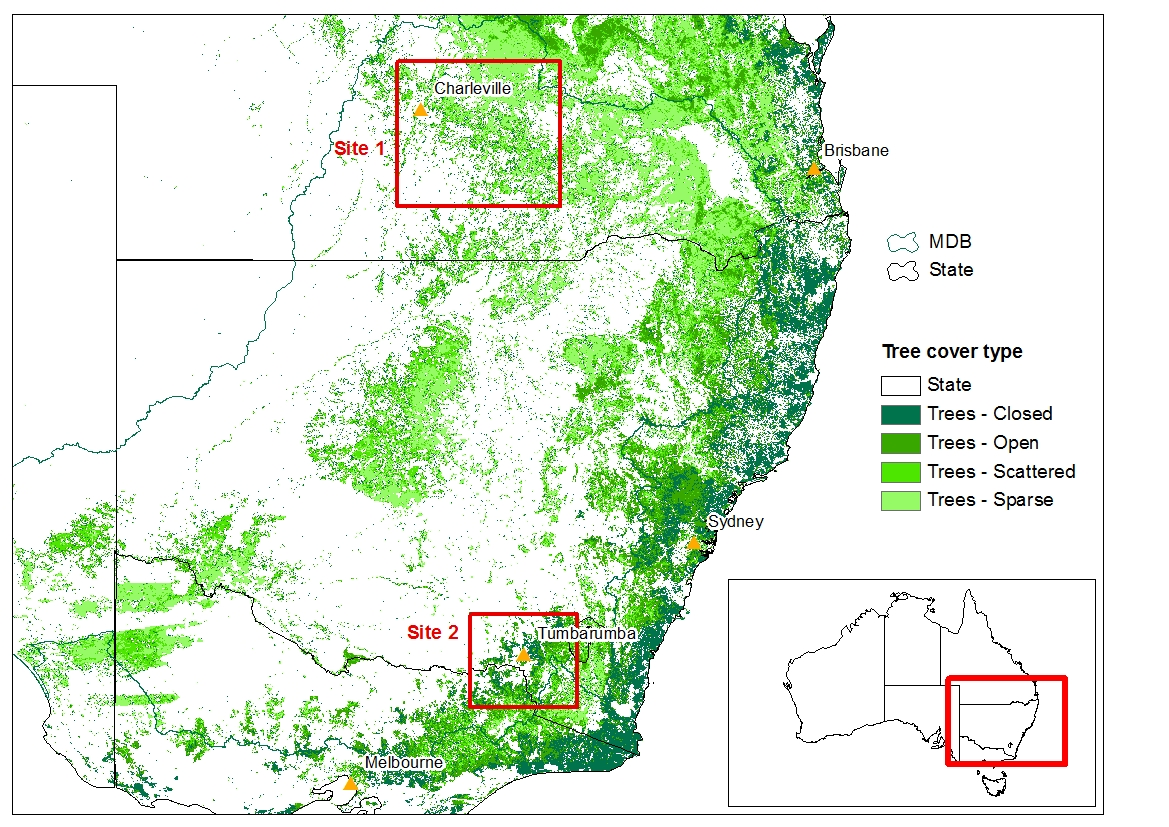
\includegraphics[bb = 8 1 800 600,scale=0.5]{map_selreg.jpg}
  \caption{Selected study regions are highlighted by red rectangles in the main map (the red rectangle in the insert indicates the location of the main map). The types of tree cover in 2008 from the DLCD product is shown at the background. In site 1 (the QLD region), the tree cover is mostly sparse. In site 2 (the NSW/VIC region), many areas have open or close forest in which tree cover is denser.}
  \label{fig:sel_reg}
\end{figure}

Two regions were selected where significant tree cover change was present. The first region is located in south central Queensland to the north of the Murray Darling Basin (MDB) (site 1 in Figure~\ref{fig:sel_reg}). High rates of land clearing have been reported in this region during the early 2000s \citep{SLATS2004}. The second study region is located at the border of New South Wales and Victoria, and includes the Snowy Mountains ranges (site 2 in Figure~\ref{fig:sel_reg}). Severe bushfires occurred in this area and the surroundings in early 2003 (see Figure~\ref{fig:bushfire}). The 2003 bushfires were the largest and the worst in this area for the last 60 years \citep{Fire2011}. Two thirds of Kosciuszko national park was heavily burned and regrowth was reported to be slow due to drought and cold conditions \citep{ABC2003} and the type of species in this region. In both study regions, significant tree cover loss has happened within the last decade, either permanently or temporarily. It makes the selected areas suitable for this land cover change study. 
%\footnote{Bushfire history, \url{http://www.dse.vic.gov.au/fire-and-other-emergencies/major-bushfires-in-victoria}, viewed on 12/12/2011}
%\footnote{Kosciuszko slow to recover from bushfires, \url{http://www.abc.net.au/news/2003-10-30/kosciuszko-slow-to-recover-from-bushfires/1501722}, viewed on 06/06/2012}

%figure 2
\begin{figure}[htp]
  \centering
  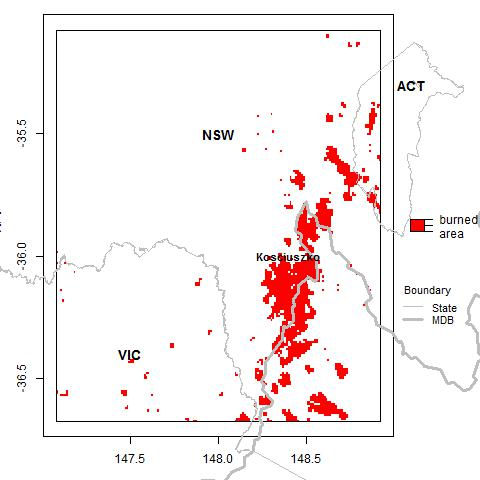
\includegraphics[bb = 1 1 500 500,clip,scale=0.6]{bushfire_nswvic.jpg}
  \caption{Location of bushfires occurring in January 2003, in and around the NSW/VIC study region, as shown by the red pixels. The map shows large area in the Kosciuszko national park has been burned. Some locations in the southwest of ACT have also experienced intensive bushfires.}
  \label{fig:bushfire}
\end{figure}

The two regions have different climate characteristics. The QLD region is partially grassland and partially subtropical, while the NSW/VIC region is mainly within the temperate zone, under the K\"{o}ppen classification. According to Australian Bureau of Meteorology (BoM), the NSW/VIC region receives 1000 - 2000 mm rainfall annually, which is more than double of the rainfall in the QLD region. Evapotranspiration is similar in both regions. Marine moisture and orographic effects are likely to be the main contributors to rainfall in the southeast mountain areas of the NSW/VIC region. 

The land use and land cover characteristics in the two regions are also different. In the Queensland region, the tree cover is sparse over most of the area. The MODIS satellite tree cover data (discussed in more detail in section 3) shows that tree cover in this region is generally below 20\% of total ground area. Grazing is the main activity in this region, with over 90\% of land used by the grazing industry \citep{ABARES2010}. Our starting assumption is that the main cause of the EVI  decline over large part of the region is due to land clearing. Tree cover has been cleared at a massive scale over the last decade, especially during 2002 - 2004. The Kosciuszko national park is within the NSW/VIC region. Here tree cover is denser with open or even closed forest (the tree cover distribution is bimodal at 10 - 20\% and 60 - 70\%). The dominant species in the alpine area are Snow Gum and large stand species such as Alpine Ash and Mountain Gum in the sub-alpine area. These trees can reach a great height but they take long time to grow. For example, Alpine Ash would need about 20 years to mature. Although land clearing is not a major issue in this region, it is vulnerable to fires and drought. 

Therefore two types of land cover changes were studied. The reports from the Queensland Statewide Land Cover and Trees Study (SLATS) \citep[e.g.][]{SLATS2001,SLATS2003} were used to investigate the time and location of land clearing in the QLD region. The MODIS burned area product, MCD45A1 \citep{Roy2002,Roy2005,Roy2008}, was used to locate bushfires areas in the NSW/VIC region, with a grid resolution of 500 m. MCD45A1 provides monthly burning information on all pixels, which helps to pinpoint an abrupt event. Due to the nature of the different land cover change, the post-change vegetation status in the two regions is expected to be different (see Figure~\ref{fig:tc_simple}). 

%figure 3
\begin{figure}[htp]
  \centering
  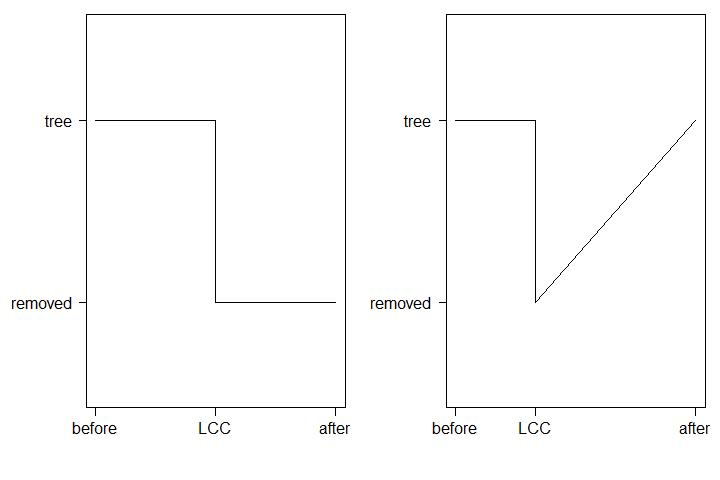
\includegraphics[bb=10 120 1000 400,scale=0.65]{tc_simple.jpg} 
  \caption{The expected evolution of the land surface after trees have been removed in (a) the QLD region and (b) the NSW/VIC region.}
  \label{fig:tc_simple}
\end{figure}




Specifically, this study focused on the effect of 2003 - 2004 land clearings in the QLD region and the effect of 2003 bushfires in the NSW/VIC region. These events are expected to cause a step change in the local rainfall. The actual tree cover change at the pixel level during this time was derived from the 11-year MODIS data (discussed below). The difference of tree cover before and after the land disturbance was tested using a Student's t-test. As the length of the tree cover data is shorter than the length of the rainfall data, earlier land clearings in the QLD region cannot be identified spatially, hence they are excluded from the analysis.

\section{Data}
\label{sec:Data}

Several land surface data sets were used in this study. The main one was the MOD44B product Global Vegetation Continuous Field dataset (version 5). This dataset provides estimates of percent tree cover (percentage of ground surface covered by trees) at a grid resolution of 250 m \citep{Townshend2011}, which is finer then the earlier mentioned burned product MCD45A1. The dataset is available on an annual time interval for the period of 2000 - 2010. The tree cover data was produced from 16-day Terra MODIS Land Surface Reflectance data and Land Surface Temperature \citep{Townshend2011}. The National Dynamic Land Cover Dataset (DLCD) \citep{Lymburner2010} from the Australian Collaborative Land Use Mapping Program (ACLUMP) was used to verify the trend of vegetation cover change calculated from the previous dataset. This dataset, developed by Geoscience Australia and Australian Bureau of Agricultural and Resource Economics and Sciences (ABARES), is the first nationally consistent and thematically comprehensive land cover reference for Australia. The DLCD is based on the 16-day Enhanced Vegetation Index (EVI), again from the MODIS satellite, between April 2000 and April 2008. It also has a grid resolution of 250 m. The dataset provides information on the final land cover types (as in 2008) and estimated trend of EVI statistics (annual mean, maximum and minimum). 

% MOD 44 - Vegetation Cover Conversion
% 
% Description:
% The MOD44 suite provides a database of land cover and change. Products are derived from 16-day composites of MODIS reflective and emissive bands at their nominal resolu-tions. The MOD44B Vegetation Continuous Fields provides 250 m sub-pixel estimates of percent woody, herbaceous and bare cover along with leaf type and longevity. The user is able to avoid constraints present in ordinal land cover maps which make a priori decisions regarding class definitions. The MOD44A Vegetative Cover Conversion pro-vides a global alarm of land cover change at a 250 m spatial resolution. Included are per-sistent change via deforestation, burning and inundation

% MOD13A3 - monthly 1 km EVI data

Rainfall data for Australia \citep{Jones2009} was obtained from BoM. The data has been projected onto a national 0.05\textdegree $\times$ 0.05\textdegree grid (approximately 5 km$\times$5 km). This gridded dataset was generated from station observations using an optimised Barnes successive correction technique. The Barnes technique combines a weighted averaging process and defined topographical information to estimate rainfall values between spatial points \citep{BoM2009}. The resulting dataset provides additional information for data-sparse areas like central Australia but reduces information in the data-rich areas, such as southeast Australia where station density is up to 20 per 100 km$^2$. The data is available on a monthly basis from 1900 to current. Here a subset of 30 years (1979 - 2008) was used. The study was conducted on monthly data, as a land cover change effect on annual rainfall might be negligible but can often found to be significant in particular months or seasons \citep[e.g.][]{Otterman1990,Gaertner2001,Semazzi2001,Oleson2004,Deo2009}. 

%% comment: in Lo2007 stated the same dataset but daily and refer the technique to Mills (1997)

Large scale climate drivers are represented by various climatic indices. The Southern Oscillation Index (SOI) is generally regarded as a good predictor of Australian rainfall \citep{Risbey2009,Chowdhury2010,Westra2010}, but its skill is weaker in some parts of Australia. For example the Southern Annular Mode (SAM) is found to be more important than ENSO in south Western Australia \citep{Meneghini2007}. The suitability of each index for the regions of interest was tested in section \ref{sec:reg_model}. The following climate indices were used as candidate predictors for local rainfall. 
\begin{itemize}
  \item Southern Oscillation Index (SOI). The Troup version of the monthly SOI series used in this study was obtained from BoM (available online at \url{http://www.bom.gov.au/climate/current/soihtm1.shtml}).
  \item Eastern, East Central and Central Tropical Pacific Sea Surface Temperatures (NINO 3, NINO 3.4 and NINO 4). Monthly SST anomalies are available from IRI/LDEO data library and the extended NINO dataset is used (available online at \url{http://iridl.ldeo.columbia.edu/SOURCES/.Indices/.nino/.EXTENDED/}).
  \item Pacific Decadal Oscillation (PDO)\footnote{Pacific Decadal Oscillation is the leading principal component of monthly SST anomaly in the North Pacific Ocean.}. The monthly PDO series was provided by JISAO (Joint Institute for the Study of the Atmosphere and Ocean, University of Washington) (available online at \url{http://jisao.washington.edu/pdo/PDO.latest}).
  \item The interaction of PDO and SOI (PDO$\times$SOI) \citep{Kamruzzaman2011}.
  %% comment: should we cite Cai et al here?
  \item Indian Ocean Dipole (IOD)\footnote{Indian Ocean dipole is commonly measured by the difference between SST anomaly in the western (50 - 70\textdegree E and 10\textdegree S-10\textdegree N) and eastern (90 - 110\textdegree E and 0 - 10\textdegree S) equatorial India Ocean \citep{Saji1999}.}. Monthly IOD was obtained from JAMSTEC (the Japan Agency for Marine-Earth Science and Technology) (available online at \url{http://www.jamstec.go.jp/frcgc/research/d1/iod/DATA/dmi.monthly.txt}).
%     \item Antarctic Oscillation (AAO). Monthly AAO series was also available from NOAA (available online at \url{http://www.esrl.noaa.gov/psd/data/climateindices/list/}).
\end{itemize}
%\footnote{BoM, 2011, \url{http://poama.bom.gov.au/data_server.shtml}, viewed on 3/1/2012}
% IOD: Saji1999



\section{Statistical method}

As shown in Figure~\ref{fig:ts_mean}, a step change is not obvious in the time series data, even though the data is deseasonalised and detrended. Hence the step changes on rainfall were analysed by two different statistical methods to provide a comparison. Both methods make use of a regression model to remove variability in rainfall hypothesised to be caused by factors other than vegetation cover change. In the first method, the tree cover change was implemented as a factor variable in the regression model. In the second method, a rank sum test (step trend test), was applied to the model residuals after effects of other major factors have been removed, assuming that vegetation cover change is the only factor explaining the non-random pattern in the rainfall residuals.

%figure 4
\begin{figure}[htp]
  \centering
  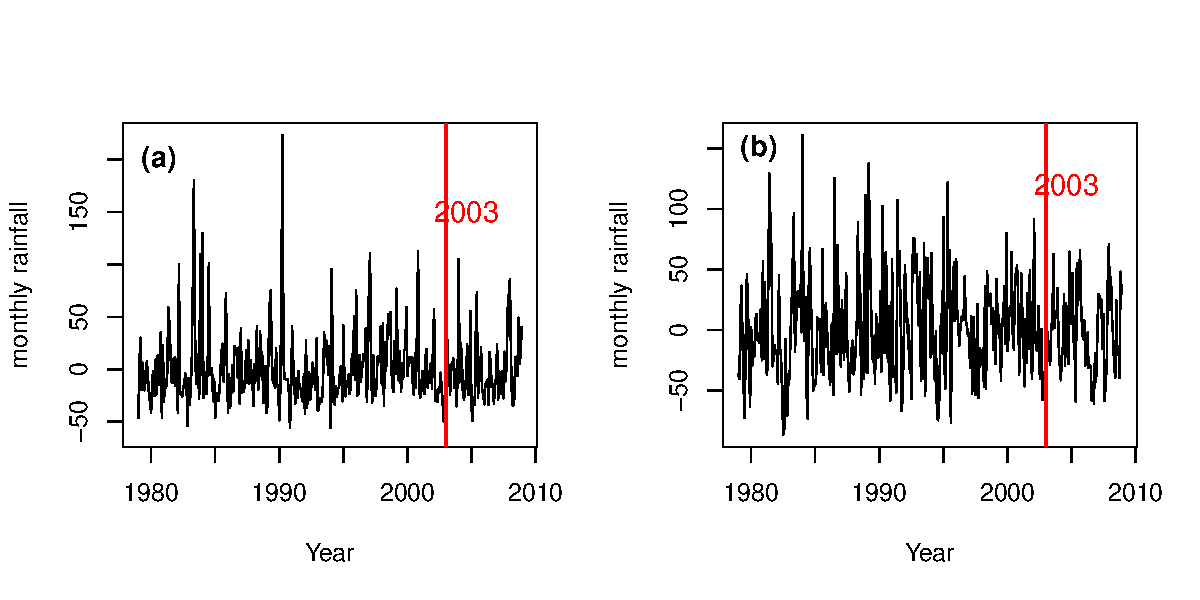
\includegraphics[scale=0.6]{mean_ts.jpg}
  \caption{The deseasonalised and detrended rainfall over the 30 years period in (a) the QLD region and (b) the NSW/VIC region. The vertical red lines indicate the year of 2003, in which the studied land cover changes occurred. A change in the time series data is not obvious before and after the land cover changes.}
  \label{fig:ts_mean}
\end{figure}

\subsection{Regression model}
\label{sec:reg_model}

Rainfall, even a single event, is generally affected by several factors. Many studies suggest the large-scale climate drivers, which are related to the global or regional atmospheric air mass movement, are the dominant control on the overall rainfall \citep{Maynard2003,DeAngelis2010,Holper2011,Smith2012}. Long term trends are shown in Australian rainfall, although whether they are due to global warming is still under discussion \citep{Wardle2004,Nicholls2006,Holper2011}.
%% comment: update references?
The difference in available radiation and hence ET in different seasons increase the variability in rainfall. The land surface effect on rainfall can be confused by changes in these factors. Hence a regression model was used to estimate the amount of variability in rainfall that is due to these important factors, and isolate changes resulting from vegetation cover change.
As highlighted in the introduction, the Australian climate is influenced by sea surface temperature in the tropical Pacific and Indian Oceans, as well as pressure systems in the Southern Ocean \citep{BoM2012}.  \citet{Risbey2009} compared five large-scale drivers, including ENSO (measured by SOI and the Tropical Pacific SSTs), IOD, SAM, MJO\footnote{MJO is a large scale eastward-propagating wave-like disturbance in equatorial latitudes \citep{Risbey2009}.} (Madden-Julian oscillation) and blocking, in relation to Australian rainfall variability. They identified SOI as the most important index among all indices tested for broad parts of Australia (including QLD and NSW/VIC) in almost any season. In this study, up to two important indices from the seven climatic indicators (see section \ref{sec:Data}) were used as the explanatory variables in the model for each study region.



As a preliminary step, the correlations between rainfall and each climatic index were analysed. Rainfall in each study region was first deseasonalised and detrended using the seasonal decomposition function ``stl" in R \citep{Rstats2011}. The reasons for using detrended data was discussed in \citet{Smith2012}. %% explain what they said
The cross-correlations between the deseasonalised and detrended rainfall and the climatic indices were tested using the Pearson's product moment correlation method, assuming the relationships are linear. Although the optimal technique for exploring the correlation with each index could be different as described in \citet{Risbey2009}, the Pearson's method was applied to all indices for consistency. Because the PDO describes the multi-decadal SST with lower frequency \citep{MacDonald2005,Zanchettin2008,Kamruzzaman2011}, instead of 30-year rainfall data, a longer period (108 years, from 1900 to 2008) was used to estimate the correlation with PDO, up to lag 24. For the other indices, the 30-year data was used. %Here lags up to 12 were applied except for PDO, for which the maximum lag was 24. 

%figure 5
\begin{figure}[h]
\centering
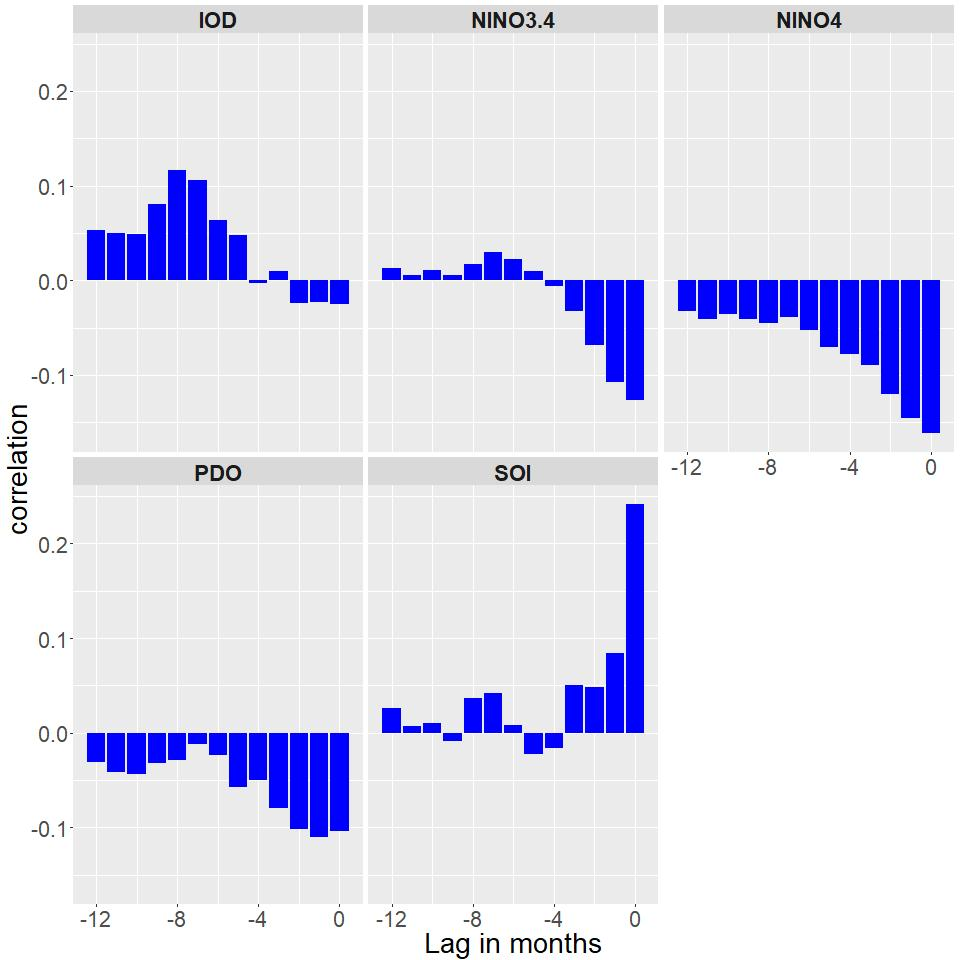
\includegraphics[bb=1 1 500 350, scale=0.6]{cor_qld.jpg}
 \caption{Cross-correlation of the six indices and rainfall in QLD study region. Where the correlations with PDO are sought, 108-year rainfall data (1900 - 2008) are used. Otherwise, 30-year rainfall data are used. The correlation with NINO 3 is not shown as it is very similar to but weaker than the case of NINO 3.4. The blue dashed lines indicate the 95\% confidence interval.}
  \label{fig:cor_rain_qld}
\end{figure}

%figure 6
\begin{figure}[htp]
\centering
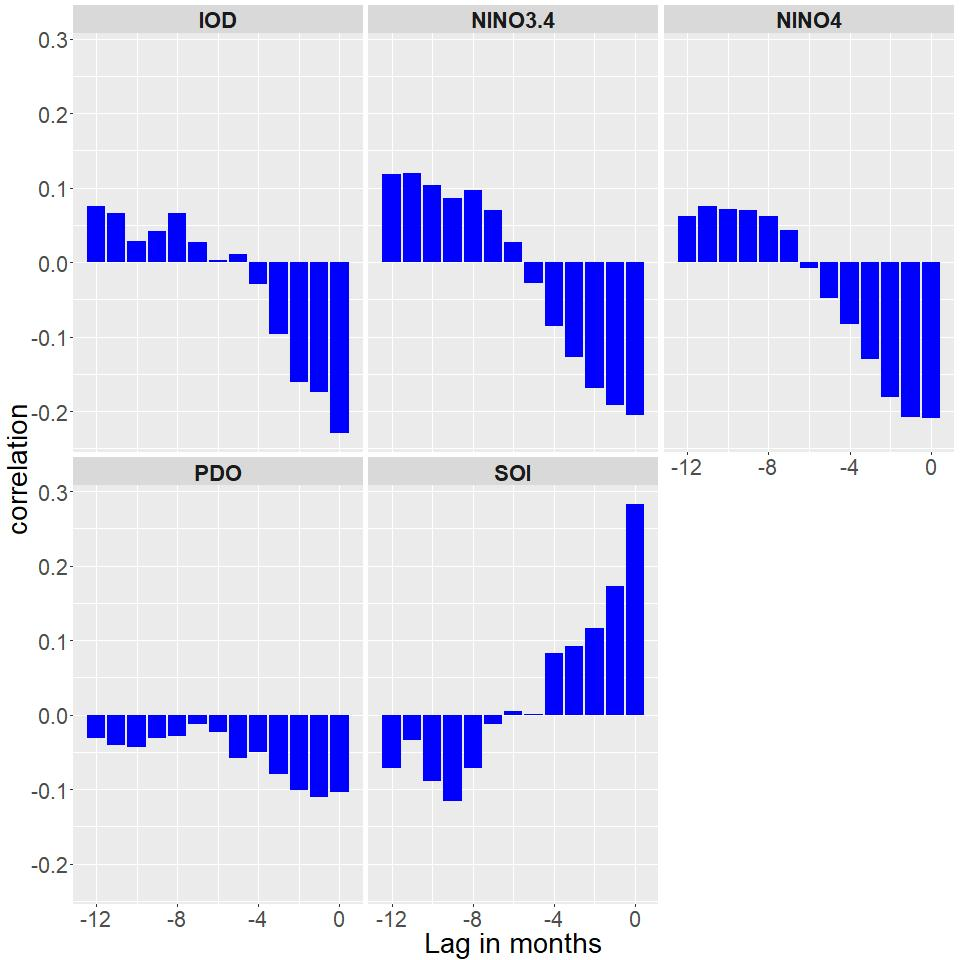
\includegraphics[bb=1 1 500 550, scale=0.6]{cor_nswvic.jpg}
 \caption{Cross-correlation of the six indices and rainfall in NSW/VIC study region.}
  \label{fig:cor_rain_nsw}
\end{figure}


Based on the correlation between the climatic indices and rainfall (as shown in Figure~\ref{fig:cor_rain_qld} and Figure~\ref{fig:cor_rain_nsw}), the following results were found:
\begin{itemize}
  \setlength{\itemsep}{0cm}
  \setlength{\parskip}{0cm}
  \item In QLD, the correlation between rainfall and SOI at zero time lags is the highest across all indices, outweighing the other ENSO indicators. 
  \item In NSW/VIC, again the SOI has the highest correlation with rainfall, followed by the IOD. Both occur at the zero time lags. 
\end{itemize}
The above findings are consistent with previous studies. Although some indices are serially correlated with rainfall up to several months, the lag zero events have the most significant correlation coefficients. Concurrent climatic index series were generally found most useful in rainfall prediction \citep[e.g.][]{Risbey2009,Kamruzzaman2011}. The correlations between the climatic indices and rainfall for each individual season have also been tested. The results were similar. So there was no change in the results as we were interested at in using no more than two indices in the model. 

%% check chamber2002 article later

Rainfall in Australia shows strong seasonal patterns \citep{Holper2011,ABS2012}. For example, the north part of the country is summer rainfall dominant with dry winter, while most of the southern part has a winter rainfall regime. This character is given by the movement of subtropical high pressure system which dominates Australian climate \citep{BoM2012a}. The seasonal component of rainfall has a periodic pattern so it is better modelled as a smooth term. A spline function was applied on the months to define a smooth seasonal pattern \citep{Wood2011}. %The spline function ``s" in R was used .

Long term trends in the regional rainfall in some parts of Australia are significant \citep{Hughes2003,Gallant2007,Chowdhury2010}. In the northern and eastern parts of the continent, increasing rainfall is reported over the last century \citep{Hughes2003}. The presence of such long term trends may be confused with the outcome of a step change in rainfall. A linear trend term was implemented in the model to remove any long term trend effect. 

We assumed all the factors are additive components in determining rainfall as in \citet{Kamruzzaman2011}. Generally, monthly rainfall has a skewed distribution so the normality assumption of the residuals in a general linear model could be violated. In this case, the rainfall model is expressed as a generalised additive model (GAM) \citep{Hastie1986} with a log link function g(), assuming the residuals are gamma distributed (see Figure~\ref{fig:hist_rain}).
\vspace{0.5cm}
%\begin{dmath}
\begin{equation}
g(E(\mathbf{R}_r)) = \beta_0 + s_1(D_{1,r}\mathbf{SOI}) + s_2(D_{2,r}\mathbf{IOD}) + s_3(\mathbf{Season}) + \beta_1\mathbf{Trend} + \boldsymbol{\epsilon}_r
  \label{eqn:model}
\end{equation}
%\end{dmath}
The bold letters represent the time series vectors. The subscript $r$ denotes the region, $r=$qld or nswvic. $\beta_u$ ($_u$=0, 1) are the fitted coefficients in the model. $s_v$ ($_v$=1, 2, 3) are the smooth functions on the climatic indices and the season. $D_{1,r}$ and $D_{2,r}$ switch on/off the corresponding climatic index in the model as discussed previously. 
\begin{equation}
  D_{1,r} = 1 
\end{equation}
as SOI was used in both regions as rainfall predictor.
\begin{equation}
  D_{2,r} = \left\{ \begin{array}{ll}
   1 &\mbox{for NSW/VIC } \\
   0 &\mbox{for QLD}
  \end{array} \right.
  \label{eqn:dummyD}
\end{equation}
The linear long term trend in the rainfall data is modelled by \textbf{Trend}=1,2,3...n, where n is the total number of months in the time series. \textbf{Season} is the seasonal component which is represented by applying a smooth spline function on the month values (1-12. The monthly rainfalls in both regions appear to have a lag 1 autocorrelation, being 0.26 for QLD and 0.33 for NSW/VIC. 
%% comment: Do we have to explain why we don't include lag 1 autocorrelation in the model, or use mixed modelling?
The SOI and IOD terms are also modelled with spline functions. As the effect of large scale drivers on Australian rainfall is more likely to be seasonal \citep{Murphy2008,Schepen2012}, the spline function can closely reproduce the high and low impacts of the climatic indices.

%figure 7
\begin{figure}[htp]
  \centering
  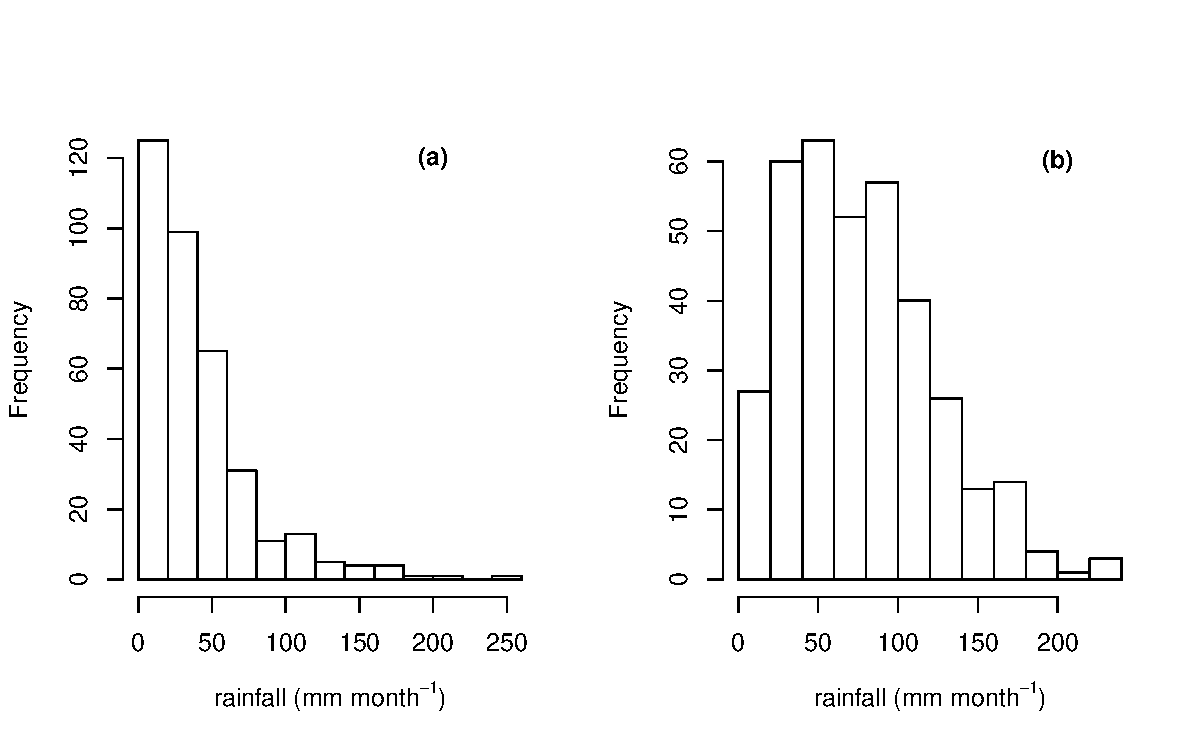
\includegraphics[bb=50 80 650 400, scale=0.6]{hist_rain.jpg}
  \caption{Distribution of monthly rainfall in (a) QLD and (b) NSW/VIC. By using a Kolmogorov-Smirnov test with shape = 1 and 2.4 respectively, rainfalls in both regions are shown to have a gamma distribution.}
  \label{fig:hist_rain}
\end{figure}

\subsection{Tree cover change as factor variable}

One of the main difficulties in empirical observation studies on the effect of land cover change on rainfall is the lack of continuous monitoring of land surface variables, or even, that no specific variable can be defined that can clearly represent the land surface process. Given the lack of a full picture of the land surface process, a factor variable was used in this study to represent the abrupt land surface change (see Equation~\ref{eqn:model2}). The change could be a result of either land clearing or bushfires as long as it is permanent or takes a long time to recover. Here we approached the problem with two different models.

In the first method, the tree cover change was used as a predictor in the regression model, represented by a factor variable \textbf{LC}. The significance of the coefficient of \textbf{LC}, denoted as $\beta'_5$ in Equation~\ref{eqn:model2}, can be determined by a ratio test. 
\begin{equation}
  \mbox{LC} = \left\{ \begin{array}{ll}
     \mbox{Trees} \\
     \mbox{Removed}
  \end{array} \right.
  \label{eqn:dummyC}
\end{equation}
Therefore in both regions, land cover is ``trees" for the period before land cover change and ``removed" for the period after the change. Here we simply assumed that vegetation cover change has occurred on every pixel. The remaining term $\epsilon_r$ is the amount of rainfall that is attributed to other unspecified factors and random errors. Hence the regression model becomes
\vspace{0.5cm}
%\begin{dmath}
\begin{equation}
g(E(\mathbf{R}_r)) = \beta'_0 + s'_1(D_{1,r}\mathbf{SOI}) + s'_2(D_{2,r}\mathbf{IOD}) + s'_3\mathbf{Season} + \beta'_1\mathbf{Trend} + \beta'_2\mathbf{LC} + \boldsymbol{\epsilon'}_r
  \label{eqn:model2}
\end{equation}
%\end{dmath}

%The valid time lengths are different in the two regions. In the QLD region, the exact timing of tree clearing is unknown. The information given in SLATS showed that clearings had occurred within 2003 - 2004. Hence in the analysis, the time series from 2003 to 2004 were discarded as the \textbf{LC} value for these two years cannot be determined. In the NSW/VIC region, severe bushfires were reported in January 2003. Storms and flooding were also reported immediately after the fires up to March in the Alpine Shire, Victoria, which could be an aftermath effect of the bushfires \citep{Tryhorn2008}. In this case, regression was performed on the time series excluding January - March 2003 to reduce the noise of storm events. The regression model was run starting from 1979 in both regions, by assuming the land covers before 2000 were ``trees".

Vegetation cover changes occurred at different times in the two regions. In the QLD region, there no exact time can be assigned to the land clearing. Clearing has occurred between 2003 - 2004 according to SLATS reports. The information on the change in type of land cover during this time period is missing. Therefore, four scenarios were tested in the analysis. In these scenarios the ``after change" period started from: (1) June 2003, (2) January 2004, (3) June 2004 and (4) January 2005. In the NSW/VIC region, severe bushfires were reported in early January 2003. Hence the ``tree" cover state was up to December 2002 then it was changed to ``removed" state from January 2003. The regression model was run from 1979 for both regions.
% Storms and flooding were also reported immediately after the fires up to March in the Alpine Shire, Victoria, which could be an aftermath effect of the bushfires \citep{Tryhorn2008}. In this case, two scenarios were tested, setting January 2003 and April 2003 as the beginning of the after-change period. 

% comment: missing values and gaps in data are complicating issues and require careful consideration \citep{Kundzewicz2004}
%comment: Hence it was assumed that clearing was at the regional scale. The land surface cover in each individual pixel is homogeneous. 

 


\subsection{Step trend test}

A step trend test was used to detect changes in rainfall after the vegetation cover change. This nonparametric statistical test was modified from the Mann-Whitney Rank-Sum test by \citet{Hirsch1985}. The test was developed to look for a step change in data which is cross correlated. The gridded rainfall dataset was built by an interpolation method and as a result there is high spatial correlation between neighbouring pixels. Hence the step trend test is suitable for the analysis of such a dataset. The advantages of this test are: (1) it does not depend on assumptions of the data distribution; (2) it is not restricted to datasets with no missing data; (3) it is robust and not as easily influenced by outliers and negative numbers \citep{Hirsch1985}.

\subsubsection{Rainfall residuals} %% do we need this heading?

The rainfall residuals from the regression model in Equation~\ref{eqn:model} were used for this test. According to \citet{Hirsch1985}, using deseasonalised and detrended data is important in a test to detect step change. Furthermore, since rainfall is only partially attributed to local sources and conditions, noise can be introduced by large scale dynamics and changes in other climatic factors. The assumption is that the regression model should remove this noise. Hence the model residuals $\epsilon'_r$ excludes the effects due to climate drivers, seasonality and the long term trend. As a result local effects are assumed to explain at least part of the variation in the residuals. The  test, described in the following sub section, associates changes in rainfall trends with the tree cover changes. 
%The step change of tree cover were expected to be identified from the rainfall residuals. 
%However deseasonalisation is unnecessary as the test was set up to count for the difference between months. Here the season term was not used in the model to reduce the risk of overfitting \citep{Wood2011}. 

%chunk 5: note code has changed

\subsubsection{Mann-Whitney rank-sum statistic}

The step trend test is a modified version of the Mann-Whitney rank-sum statistic \citep{Hirsch1985}. As a nonparametric rank-based test, the Mann-Whitney test does not use the exact values of rainfall but depends on the ranks of the data. For each month, rainfall residuals of each year were ranked in an ascending order. The ranking of January rainfall in a sample pixel k in QLD is illustrated below:\\

%\begin{table}[h]
%  \centering
  \begin{tabular}{lccccccc}
  & 1998 & 1999 & 2000 & 2001 & 2002 & 2005 & 2006\\
  \textit Rainfall residuals: & -0.3 & -60.9 & -16.1 & -71.7 & 111.1 & -7.2 & -60.5 \\
  \textit Rank ($R'_{1k}$): & 6 & 2 & 4 & 1 & 7 & 5 & 3\\
  \end{tabular}
%\end{table}
\noindent Therefore, the smallest or most negative value has rank 1 and the largest value has the maximum rank.

The before period and the after period formed two groups of samples. The split point of the two periods was based on the timing of the vegetation cover changes. In the QLD region, changes occurred anytime during 2003 and 2004. In contrast to the previous method, the time period of where the land cover chang occurred was excluded, as the nonparametric test allows missing data. \citet{Hirsch1985} also pointed out that the power of the test is higher if the data of the change period is ignored. Hence 2003 and 2004 were excluded from the analysis. As a result, the after-change period was 2005 - 2007. 

In the case of NSW/VIC, the bushfires broke out in early January 2003. The change was within a relatively short period of the year. Therefore the after-change period in this region still started in January 2003. Following \citet{Hirsch1985}, the before period was set to five years (1998 - 2002) in both regions. %The test does not require a long time series before and after the intervention as shown in \citet{Hirsch1985}.
  
The rank of rainfall in month j year i in pixel k is denoted as $R'_{ijk}$. The sum of ranks of rainfall in month j in pixel k before the known intervention is:  
\begin{equation}
  W_{jk} = \sum_{i=1}^{n_1}R'_{ijk}.
  \label{eqn:Wj}
\end{equation}
$n_1$ is the number of years before the land cover change. The expected value of $W_{jk}$ is 
\begin{equation}
  \mu_w=n_1(n_1+n_2+1)/2
\end{equation}
$n_2$ is the number of years after the change. Hence the expected value of the rank sum before the intervention is the same for all months and all pixels. The sum of ranks for the whole time period is fixed, as $(n_1+n_2)(n_1+n_2+1)/2$. In this study, since there are only two groups (before and after), knowing the rank-sum of one group is the same as knowing the rank-sum of the other group. If the rainfall data is temporally and spatially independent, the variance of $W_{jk}$ is 
\begin{equation}
  \sigma^2_w = n_1\cdot n_2(n_1+n_2+1)/m
\end{equation}
where m is the number of months which is 12 in the case of a full year. 

\subsubsection{Step trend test}

Instead of completing the Mann-Whitney U-test, \citet{Hirsch1985} applied the rank-sum statistics in a standard normal Z test. The modified test can be used to detect step change and it accounts for serial and cross correlation in the data. In the case here, the deseasonalised and detrended data shows little autocorrelation in the time series but possesses strong cross correlation between neighbouring pixels, i.e. $R>0.99$. Hence the covariance between pixels would need to be considered in the test.

% Assuming the distribution of $W_{jk}$ is normal and independent, 

The sum of $W_{jk}$ for a block of $ns$ pixels over the whole year, $\sum_{j=1}^{12}\sum_{k=1}^{ns}W_{jk}$, has mean 
\begin{equation}
  E(\sum_{j=1}^{12}\sum_{k=1}^{ns}W_{jk})=12\cdot ns\cdot\mu_W
\end{equation}
and variance
\begin{equation}
  Var(\sum_{j=1}^{12}\sum_{k=1}^{ns}W_{jk})=\sum_{j=1}^{12}\sum_{k=1}^{ns}\sum_{h=1}^{ns}C(W_{jk},W_{jh}).
\end{equation}
$C(W_{jk},W_{jh})$ is the covariance of the W statistics between pixel k and pixel h in month j. When $k=h$, $C(W_{jk},W_{jh})=\sigma^2_w$. When $k\neq h$, 
\begin{equation}
  C(W_{jk},W_{jh})=\sigma^2_w r(R_k,R_h)
\end{equation}
where $r(R_k,R_h)$ is the product moment correlation coefficient of the concurrent ranks in pixel k and h. Here $r$ is calculated on the full time series in each pixel. In this analysis, the test was applied to a square block of four pixels each time. As argued by \citet{Hirsch1985}, $ns=4$ is the most optimal solution to balance the cost and the gain in the test power.
% \begin{equation}
%   \sigma^2_{w12} = 12\cdot\sigma^2_W = n_1\cdot n_2(n_1+n_2+1).
% \end{equation}

The statistic of the step trend test is then defined as 
\begin{equation}
  Z'=\frac{\sum_{j=1}^{12}\sum_{k=1}^{ns}W_{jk}-12\cdot ns\cdot\mu_w}{\sqrt{Var(\sum_{j=1}^{12}\sum_{k=1}^{ns}W_{jk})}}.
  \label{eqn:Z}
\end{equation}  
The above statistic is written for a 12 month period. By changing the value 12, it can also be used to test seasonal rainfall change or for other customized periods.

%The Z' test is based on the assumption that the sum of $W_j$ is normally distributed. Small numbers of $n_1$ and $n_2$ might weaken this assumption. On the other hand, because there is a much longer period before the intervention in the rainfall data, the possible changes at some other time could increase the noise in the analysis. Given the rainfall time series data was only available up to 2008 and the specified land intervention was closer to the end of this time series, a subset of the rainfall time series was selected from 1998 to 2008. This 11-year rainfall data analysis was compared to the time series analysis for the full period. 

The null hypothesis ($H_0$) in this study is that there was no change in rainfall due to land surface intervention. The results of the step trend test can be interpreted according to the sign of Z' score (see Table~\ref{tab:Zscore}). Z' is normally distributed similar to the standard normal statistics Z. Hence it can be compared to a standard normal distribution to determine the p value. 

\begin{table}
  \caption[The interpretation of Z' score in the step trend test.]{The interpretation of Z' score in the step trend test. Following \citet[][Chapter 23, P887]{Hipel1994}.}
  \label{tab:Zscore}
  \centering
  \begin{tabular}{|l|l|} \hline
    Z' $>$ 0 & rainfall decreases after change\\ \hline
    Z' $<$ 0 & rainfall increases after change \\ \hline
    Z' = 0 & rainfall does not change \\ \hline
  \end{tabular}
\end{table}
  
%chunk 6

% chunk 7: bootstrapping (do not keep spatial structure, not in use)

% chunk 8: bootstrapping (spatial structure is kept, in used)

% chunk 9: bootstrapping (spatial structure is kept, remove short term trend, randomly select after change period)
%% apply the LocSig function in SpatialVx for block bootstrapping


\section{Result}

\subsection{Tree cover changes}

The pixels with significant tree cover change in each study region are shown in Figure~\ref{fig:tc_trend}, at the 0.05 significance level. Given the limitation of the length of this data series, it still indicates a large change in the NSW/VIC region. In the NSW/VIC region, much of the tree loss between 2002 and 2003 was concentrated in the Snowy Mountains which are at the border of NSW and VIC. Tree cover loss occurred in large parts of the QLD region between 2002 and 2005. Most of the clearings appear in the centre of this region. The tree cover change map is consistent with the annual mean EVI trend map (based on DLCD data, map not shown here), which confirms these changes are significant and persistent over the study period. 

%figure 8
\begin{figure}[htp]
\centering
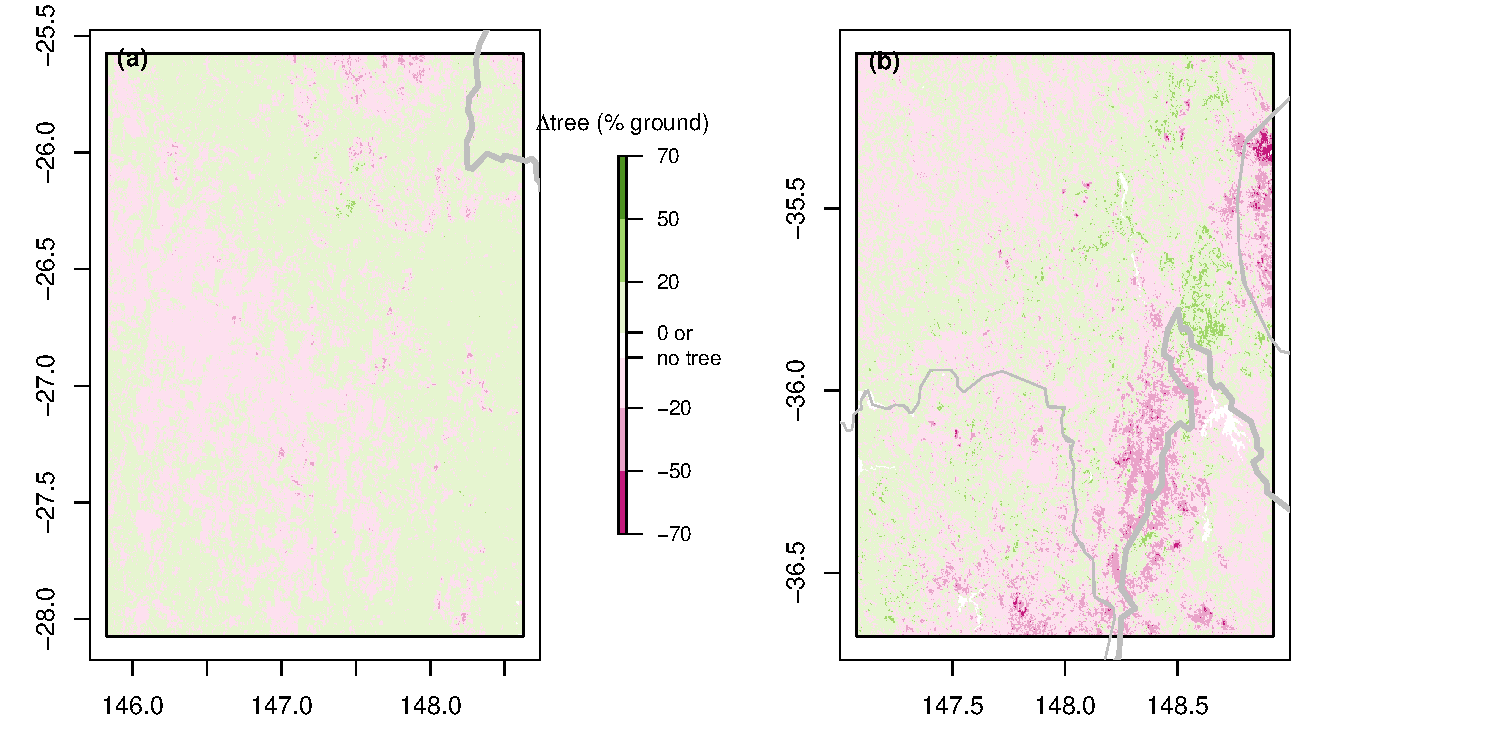
\includegraphics[scale=0.65]{tc.jpg}
  \caption{The maps show the areas with significant changes in tree covers in (a) the QLD region and (b) the NSW/VIC region. The amount of changes was calculated as the difference in tree covers before and after the specified land cover intervention and it is shown as the percentage of the ground area. Green colour indicates an increase in tree cover, while red colour indicates a decrease in tree cover. }
  \label{fig:tc_trend}
\end{figure}

\subsection{Regression Model \& Significance of Vegetation Cover Changes}

The regression model does not explain much of the rainfall variability. The model in Equation~\ref{eqn:model2} accounts for around 13\%\footnote{Here the adjusted $R^2$ was reported. Adjusted $R^2$ is the coefficient of determination, a measurement of the amount of variability predicted by the model adjusting for the number of explanatory terms} of the rainfall variations in the QLD region and 19\% in the NSW/VIC region on average. The residual analysis shows that the assumptions of the regression model are generally met. The standardised residual plots, however, show some funnelling for the NSW/VIC regions, suggesting non constant variance. The residual analysis, based on one sample pixel from each region, in Figure~\ref{fig:residuals_qld} and Figure~\ref{fig:residuals_nswvic} illustrates this. The residual patterns are consistent within each region.
% Can Fig9 and Fig10 be combined?
%Later when the land cover variable was excluded the results were similar as this variable can only represent a small variation in the data.
%Furthermore, the model residuals in NSW/VIC is random and normally distributed, while it is close to normal in QLD. 

The model confirms the importance of the climate drivers and the seasonality in Australian rainfall. Even at the grid level, the seasons and the climatic indices were significant ($\alpha = 0.05$) everywhere in both regions. The explaining power of the model is mostly due to these variables. The climate drivers (at lag zero) accounted, on average, for 6\% of the rainfall variability in both the QLD region and the NSW/VIC region (see Figure~\ref{fig:rsq} for the distribution of $R^2$ in these two regions). These figures are within the upper bound of seasonal rainfall predictability by SST anomaly field reported by \citet{Westra2010}.

%figure 9
\begin{figure}[htp]
  \centering
  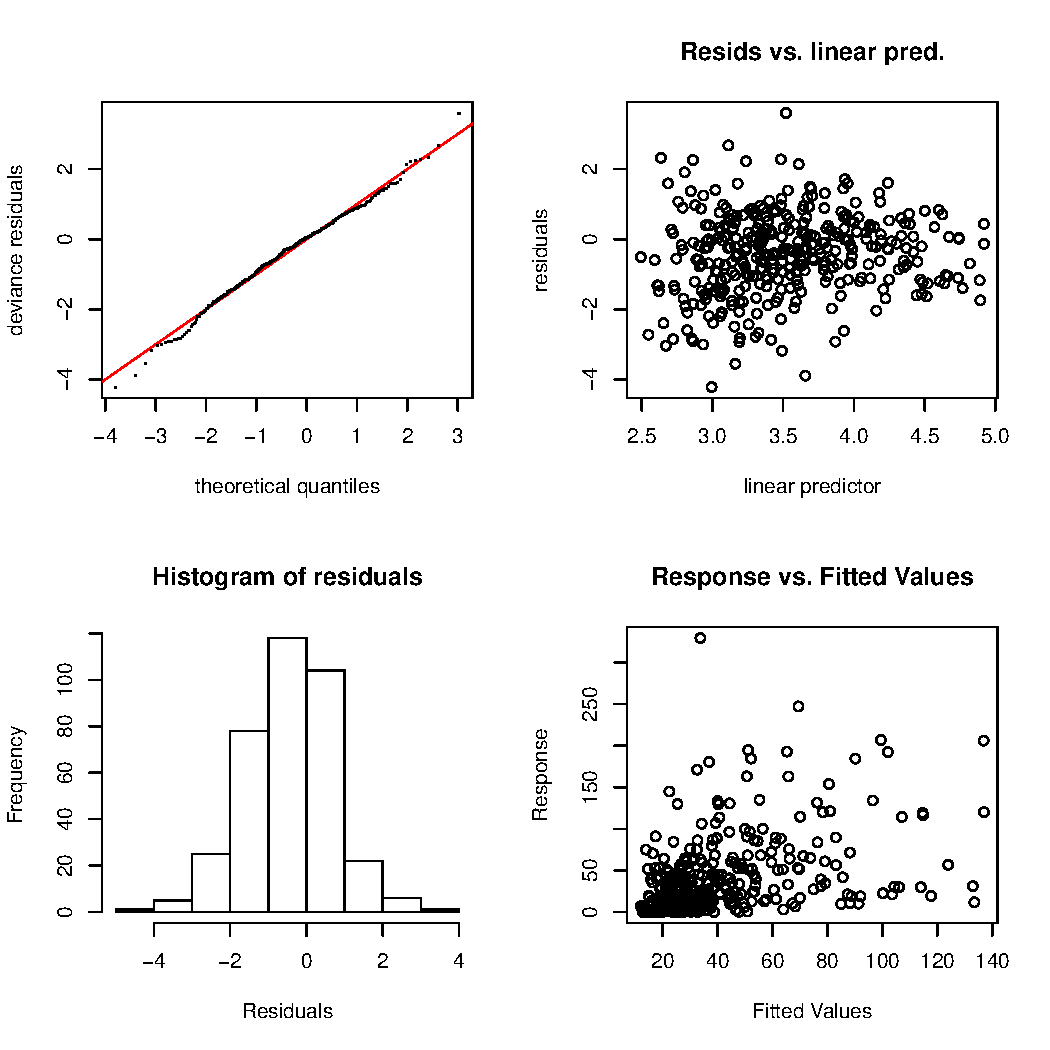
\includegraphics[bb=0 0 650 500, scale=0.8]{qld_check.jpg}
  \caption{The residual analysis of a sample pixel in the QLD region.}
  \label{fig:residuals_qld}
\end{figure}

%figure 10
\begin{figure}[htp]
  \centering
  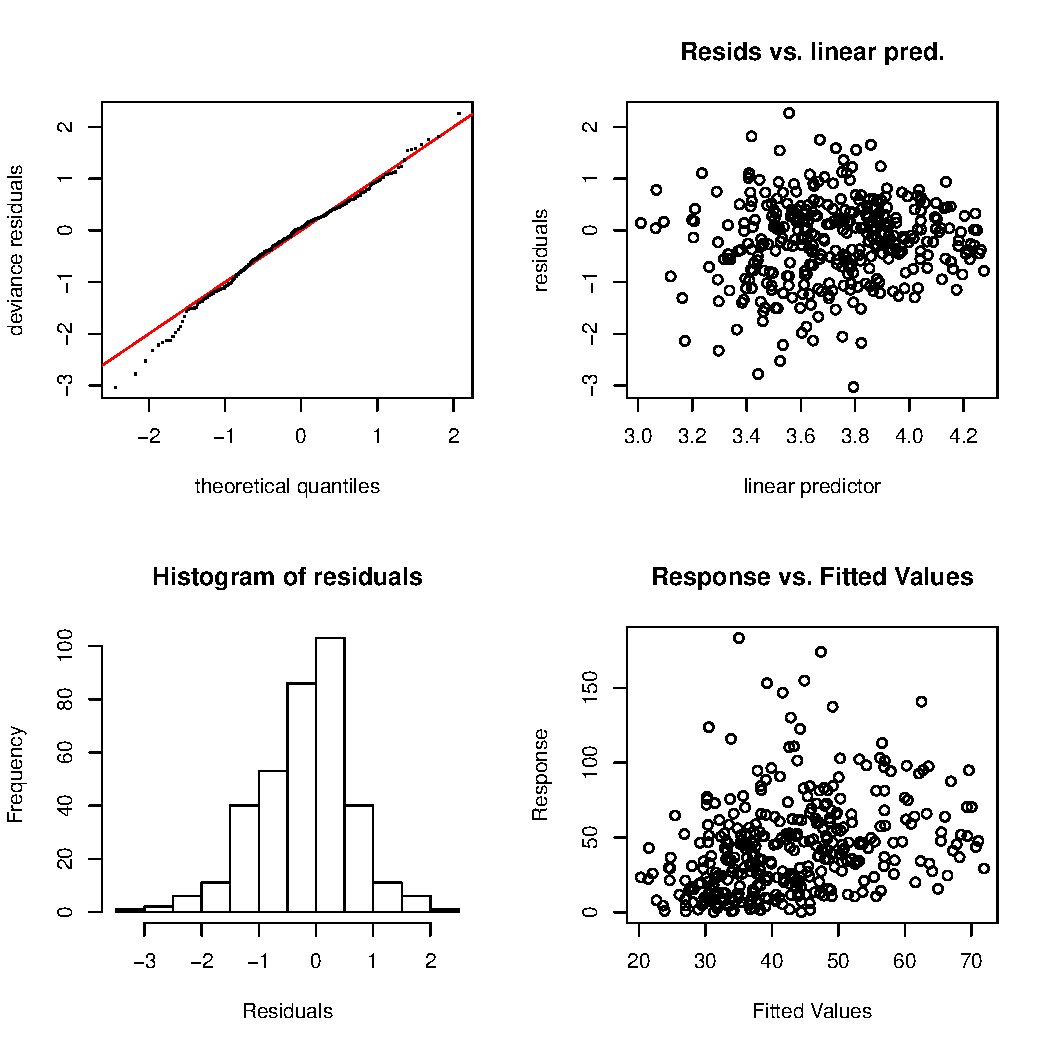
\includegraphics[bb=0 0 650 500, scale=0.8]{nswvic_check.jpg}
  \caption{The residual analysis of a sample pixel in the NSW/VIC region.}
  \label{fig:residuals_nswvic}
\end{figure}

%figure 11
\begin{figure}[htp]
  \centering
  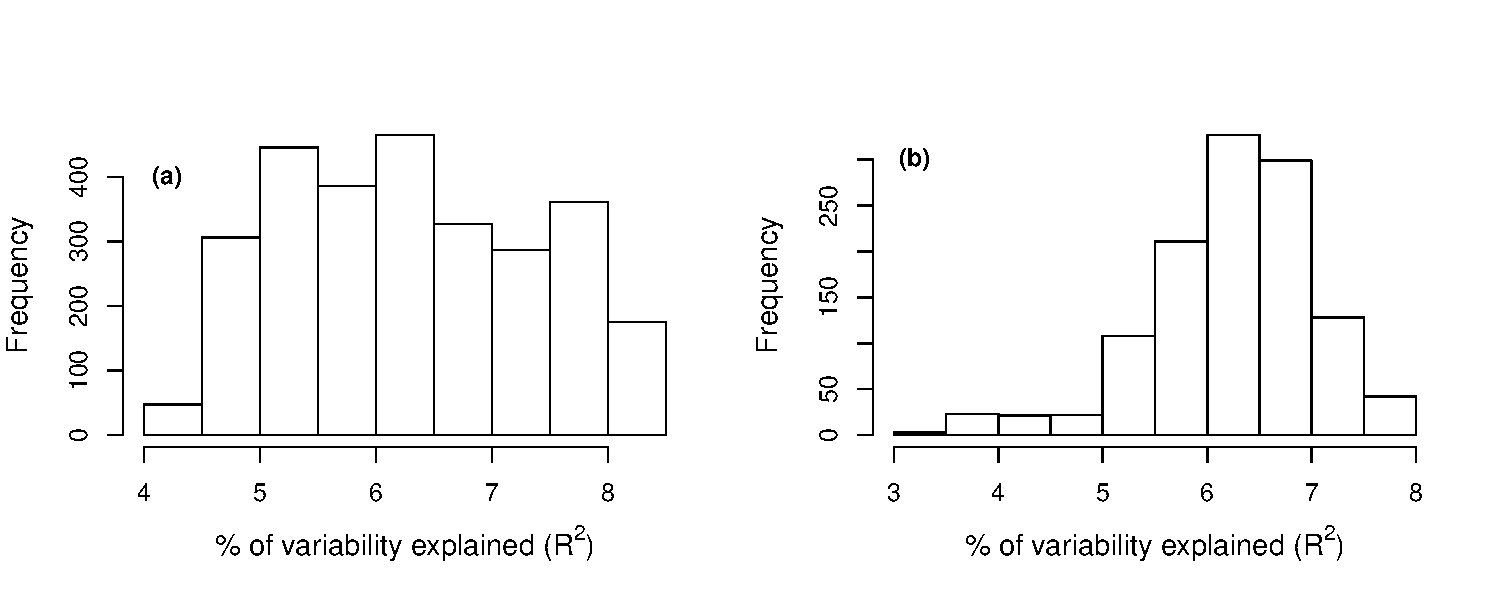
\includegraphics[bb=0 100 960 500,scale=0.65]{soi.jpg}
  \caption{The distribution of $R^2$ when rainfall is only modelled by the climate drivers. It shows the percentage of rainfall variability that can be explained by the climate drivers. In the case of (a) the QLD region, SOI was the only climatic index considered. In (b) the NSW/VIC region, SOI and IOD were used.}
  \label{fig:rsq}
\end{figure}


A statistically significant long term trend was not observed in either of the two regions. However, this result might not disprove the importance of a long term trend in rainfall. The overall time period is farily short and more pixels in NSW/VIC would have significant step change if the long term trend effect is not removed by the model. As trend free data is an important requirement for the step trend test, the trend term was kept in the regression model to ensure the detection of step change was not due to a possible long term trend. 

%figure 12
\begin{figure}[htp]
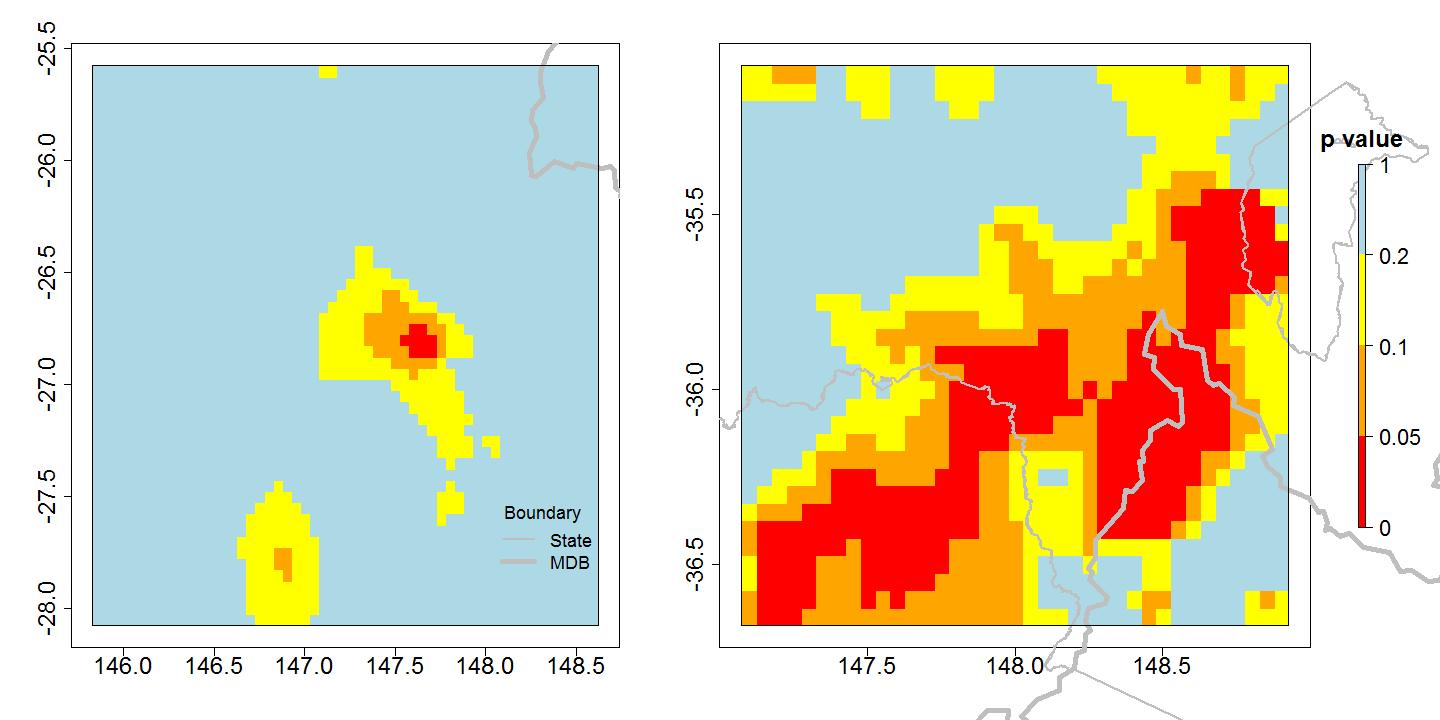
\includegraphics[bb=10 50 960 500, scale=0.6]{Cp_30yrs.jpg}
  \caption{The spatial distribution of significance of vegetation cover changes in the two study regions. The significance of vegetation cover changes is assessed in the regression model. The figures report the p values of the coefficient of the land cover variable in the model at different significance level. The plot of the QLD region is for the scenario that the after change period started from January 2005, as the other scenarios have no p value less than 0.2.}
  \label{fig:LC_p}
\end{figure}

The land cover variable implies a step change with different values before and after the land cover intervention. This variable was only significant ($\alpha=0.05$) for the rainfall estimates in some areas in NSW/VIC, as shown in Figure~\ref{fig:LC_p}~(b). The effect of tree removal in the NSW/VIC region was highly significant in the area from the Snowy mountains ranges in the south to the west side of Australian Capital Territory (ACT), highlighted by the red colour in Figure~\ref{fig:LC_p}~(b). However no significant step change due to the land cover changes was found in rainfall of the QLD region in any of the four scenarios. 

In the NSW/VIC region, the locations of rainfall change show some agreement with the locations of vegetation cover change. Comparing the results in Figure~\ref{fig:LC_p}~(b) to Figure~\ref{fig:tc_trend}~(b), the alpine area with massive tree cover loss is located inside the highlighted region. The results show that the step change in rainfall also occurred in the cotter river catchment which was heavily burned in 2003 bushfires (refer to Figure~\ref{fig:bushfire}). However, Figure~\ref{fig:LC_p}~(b) also shows that significant step change in rainfall was found in an area larger than where the bushfires has occurred. From this point of view, the results might be showing a large scale effect that reaches beyond the vegetation cover change effect. %A close look at the rainfall data revealed that it was very low in 2006, which corresponds to a severe drought due to a weak El Ni\~{n}o and unrecovered condition from the previous drought. %this area does not show up in the tree cover change map. The post-fire revegetation and restoration activities in ACT could have reduced the significance of the difference in tree cover before and after the bushfires. It is an indication that deforestation might cause a step change in rainfall but reforestation could take a long time to show effects.

%Due to the uncertainty in the timing of the land clearing, in this experiment different time windows for land clearing have also been tested. Little influence of land cover change effect was found if the time window was changed to 1990 - 2004. If the time window was between 2000 - 2004, the spatial distribution of the p value was similar to Figure~\ref{fig:site1_p}. If the time window included 2005, the results suggested that rainfall has been affected by land cover change over an even larger area on the east. This area also corresponds to the area where a high rate of clearing in 2005 - 2006 was reported \citep{NaturalResources2008}. However the confidence level of the results also decreased as this change further reduced the length of years after the land intervention in the analysis.

More generally, the model also shows that the tree cover has a positive impact on rainfall. The fitted coefficients for the reference state ``trees" were consistently positive for the pixels whose step changes of rainfall were significant. It implies that rainfall was higher when the surface was covered by trees. This was confirmed by applying a two sample Student's t-test on the annual rainfall of the before-change and after-change periods. %With a maximum coefficient value of 0.36, the magnitude of difference between the two states appears to be small.

\subsection{Step Trend Test}

%figure 13
\begin{figure}[hpt]
  \centering
 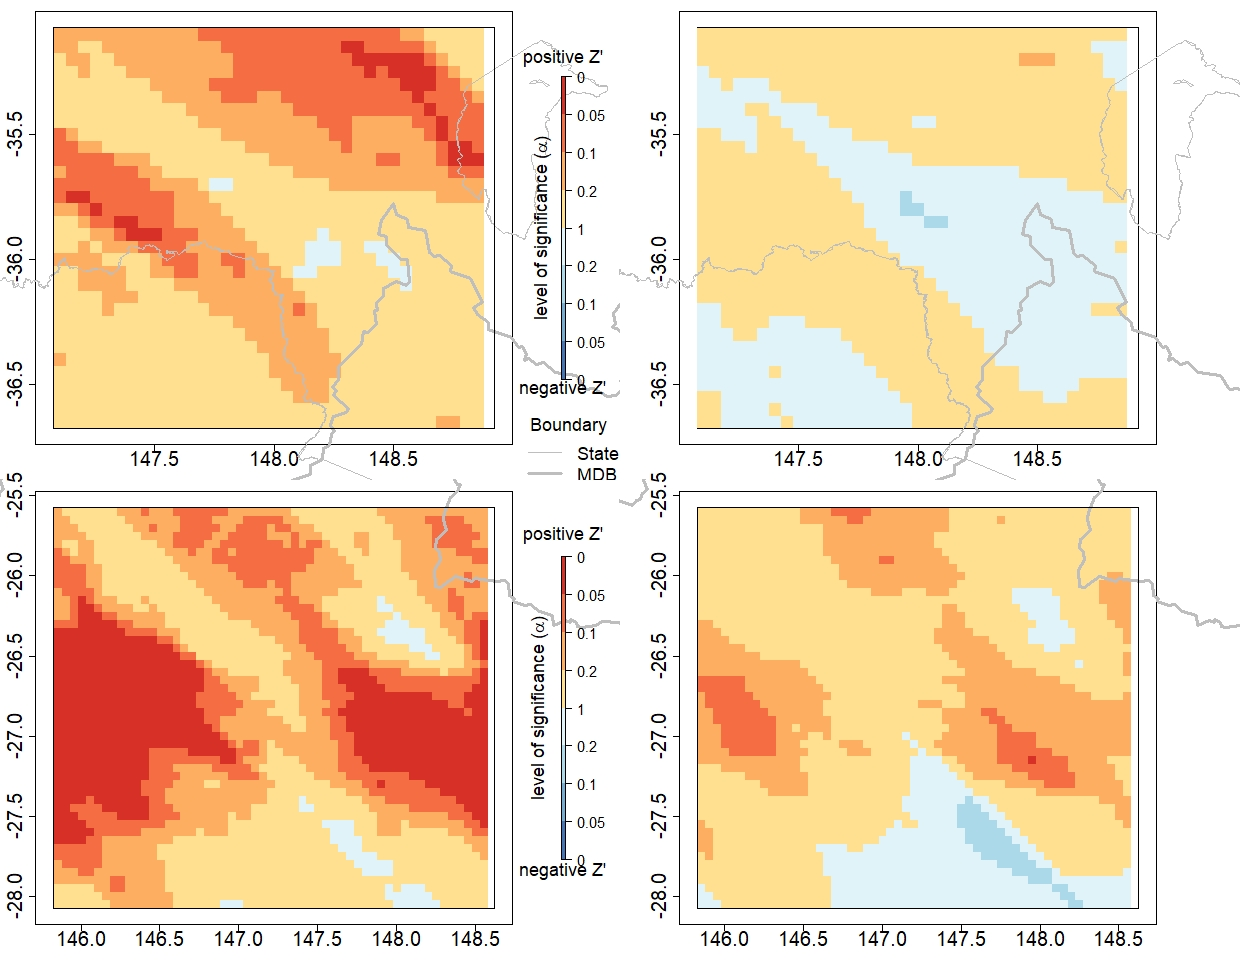
\includegraphics[bb=0 80 960 500, scale=0.7]{step_new.jpg}
  \caption{Spatial distribution of the step trend test Z' statistics in the two study sites. The test was conducted on the 30-year rainfall data from 1979 to 2009. Warm colours (yellow, orange and red) are for positive Z' values which indicate decreasing rainfall trend due to the land surface intervention. Cold colours (light blue to blue) are for negative Z' values which indicate increasing rainfall trend. The deeper the colour, the more significant the statistic.}
  \label{fig:steptest30}
\end{figure}

The spatial step trend test Z' scores are shown in Figure~\ref{fig:steptest30}. This figure provides two types of information: the sign and the significance level. The sign indicates the direction of the step change, as listed in Table~\ref{tab:Zscore}. In each region, there is a broad area of positive Z' values which implies a decrease in rainfall. In QLD, the areas of positive Z', especially when $\alpha$ is smaller than 0.1, almost align with the locations reported to have heavy land clearing (see Figure~\ref{fig:slat}). However the vegetation cover change map in Figure~\ref{fig:tc_trend}~(a) does not clearly show a similar pattern. In the Snowy Mt area and the west of ACT, where severe bushfires occurred in 2003, positive Z' values were found. It again indicates that loss of tree cover appeared to be related with a rainfall decrease. Nevertheless the observed step change in rainfall was not strong. At the 5\% significance level, changes in a number of pixels in the alpine area are possibly where the tree recovery is slow. In the QLD region, 35 pixels obtained a Z' score with p $<$ 5\%. In the NSW/VIC region, there are only 18 pixels in the alpine area having a Z' score with p $<$ 5\%. They are a very small proportion of both study regions.
% should we also report p $<$ 10\%?
%Although the rainfall changes were not significant, the spatial patterns of the positive Z' scores agree with the nature of the tree cover change in these two regions. This is again showing the possible regional effect of the land cover changes, which is consistent with the results from the regression analysis. 

%figure 14
\begin{figure}[htp]
  \centering
  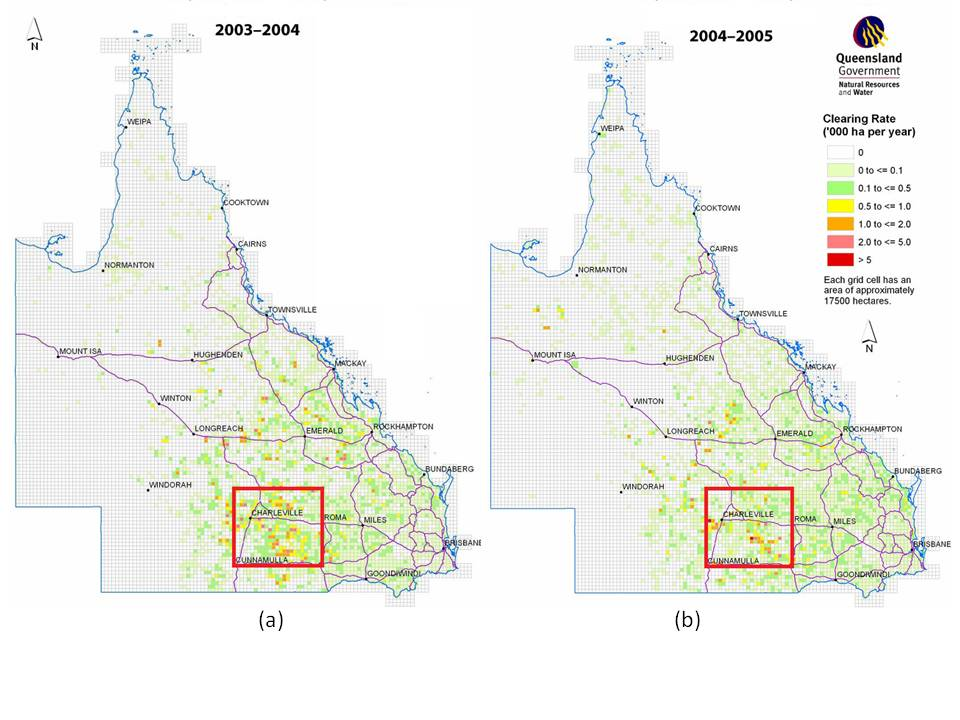
\includegraphics[scale=0.6]{slat.jpg}
  \caption{Woody vegetation clearing rate in QLD. The maps and figures are obtained from \citet{SLATS2004}. The red rectangle is the boundary of the QLD study region.}
  \label{fig:slat}
\end{figure}

%figure 15
\begin{figure}[htp]
  \centering
  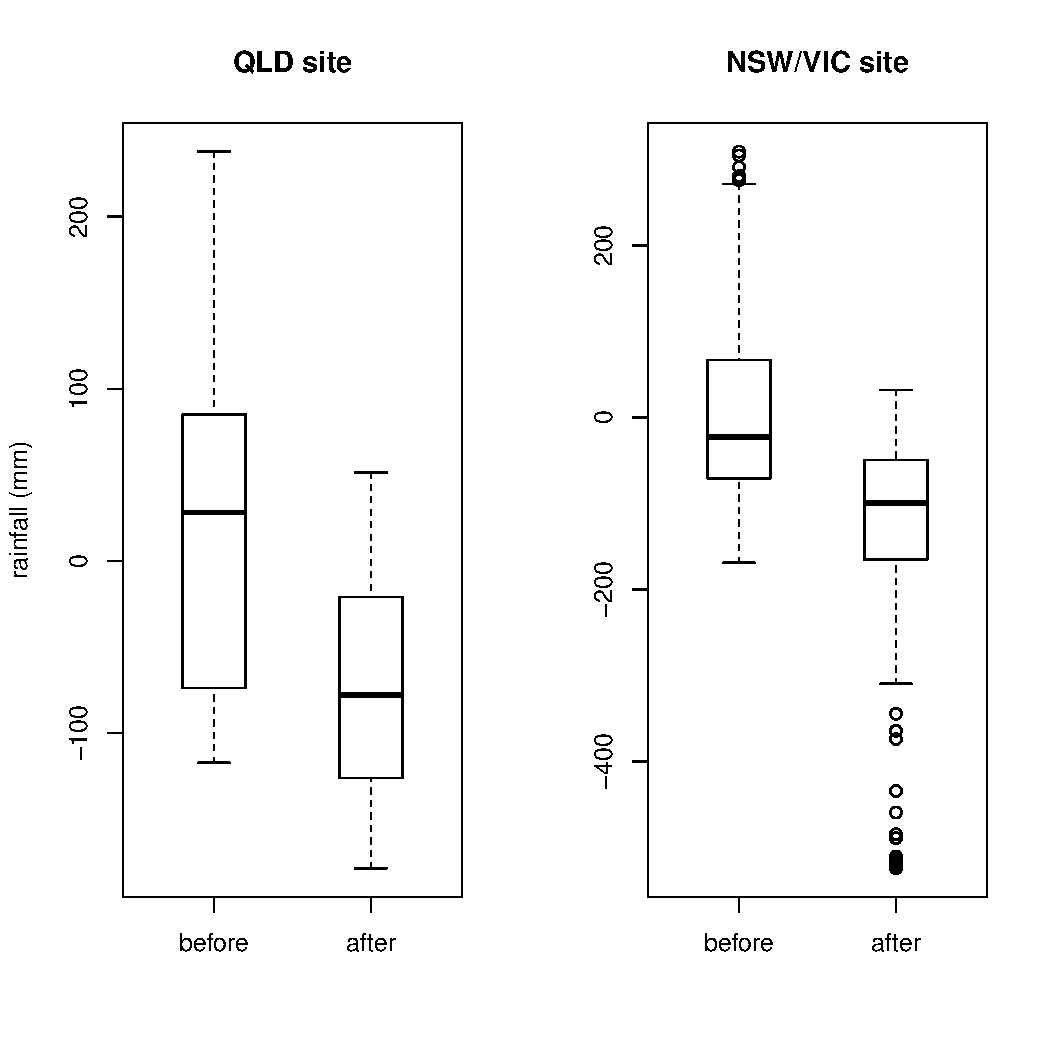
\includegraphics[bb=0 0 650 500, scale=0.8]{compare_mean.jpg}
  \caption[Boxplots of annual rainfall (estimated based on rainfall residuals from Equation~\ref{eqn:model}) before and after the land cover intervention during 1998 - 2008 in the study regions.]{Boxplots of annual rainfall (estimated based on rainfall residuals from Equation~\ref{eqn:model}) before and after the land cover intervention during 1998 - 2008 in the study regions. On average, the after period has a lower annual rainfall amount and with outliers of small values.}
  \label{fig:mean_diff}
\end{figure}

The rainfall residuals of the two periods (before-change since 1998 and after-change) were also compared (Figure~\ref{fig:mean_diff}). The annual values of the 11-year period (1998 - 2008) were calculated for each pixel. The boxplots indicate that there were different mean values between the ``before" and ``after" periods in both regions. There are small outliers in the after period in NSW/VIC. A close look at the rainfall data revealed that rainfall was consistently very low in 2006 for the whole region. The low rainfall in 2006 was due to a weak El Ni\~{n}o and unrecovered conditions from the previous drought. While the regression model has removed most of the effect of ENSO, the  cumulative drought effect could still be visible in the residuals if the response of the rainfall to the ENSO effect is non-linear, and the memory of the past drought is persistent. This can also explain the significant results in the previous method. To remove the outlier effects, the two periods were compared excluding the 2006 rainfall. An F test confirmed that the variances were different between the before and after periods. Hence an unpaired unequal variance two sample t-test was applied to test whether the after period has lower mean rainfall than the before period, for the group of pixels showing a negative step change in rainfall ($\alpha = 0.05$) and the group of pixels with no change. The rainfall in the after period was lower than the before period (p $<$ 0.05) for pixels showing a negative step change. For those pixels without a step change, there was no statistical evidence that the two periods have different means. Hence the t-test results are consistent with the step trend test results.
%  that showed a negative step change in rainfall ($\alpha$ = 0.1) and compared to pixels without change
%The boxplots in Figure~\ref{fig:mean_diff} indicate that the rainfall distributions in the two periods are different. 


The choice of $ns$ has some impact on the test results, as shown by \citet{Hirsch1985}. The cases of $ns = 1$ and $ns = 9$ were also tested. When $ns = 1$, 18 pixels in the QLD region obtained a Z' score at the 5\% significance level. In the NSW/VIC region, the detection of negative step change ($\alpha = 0.05$) reduced to 16 pixels. On the other hand, when $ns = 9$, the results were similar to the case of $ns = 4$. The changes ($\alpha = 0.05$) were detected in 35 pixels in the QLD region and 18 pixels in the NSW/VIC region. The power of the test does not change much after $ns = 4$, as shown by \citet{Hirsch1985}. The cause of the highly inconsistent results in the QLD region between $ns = 1$ and $ns = 4$ is unclear. This could possibly be because the higher $ns$ values smooth the individual pixel results.

The "field significance" of the test is considered to make inferences about the step change at regional scales from multiple local tests \citep{Wilks2006,Westra2013}. Here, the bootstrapping resampling method from \citet{Westra2013} was adapted , modified to evaluate the field significance. The spatial structure of the pixels was maintained, while the order of the years and months, as well as the length of the before/after windows were changed by random resampling. The test statistics identifies the percentage of the pixels with significant step change, positive and negative respectively, for the step trend test. The test statistics on 1000 resampled replicates were used to develop the distribution of these percentage values under the local null hypothesis that there was no step change.

The bootstrapping resampling technique was applied on both $ns=1$ and $ns=4$ cases. In the $ns=4$ case, a spatial moving block bootstrapping was used, in which the change of time sequence within the 2$\times$2 block was consistent. The distribution of the test statistics is highly concentrated at zero with a skew to the right. In all four outputs, positive step changes and negative step changes in the cases of $ns=1$ and $ns=4$, the test statistics on the observed time series fall within the null hypothesis distribution (the cases of $ns=1$ are shown in Figure~\ref{fig:boot_qld} and Figure~\ref{fig:boot_nsw}). The results showed that the chance of detecting a rainfall change was small. Again there was no strong evidence to support the hypothesis that vegetation cover change can affect local rainfall.
%% I think this shows that the results we got could just be by chance

%figure 16
\begin{figure}[ht]
\centering
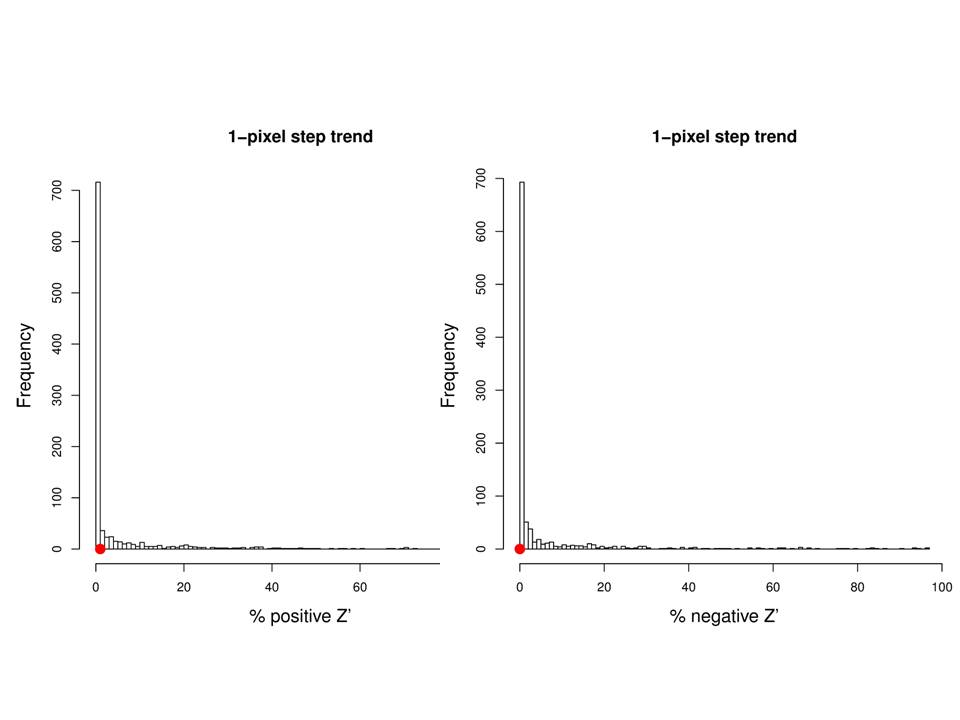
\includegraphics[width=6.5in]{bt1_qld.jpg}
\caption{Percentage of pixels showing statistically significant positive Z' values (left) and negative Z' values (right) in QLD. The histogram shows the distribution of results from 1000 bootstrap resampling of the rainfall time series. The red dot represents the results from the observed data.}
\label{fig:boot_qld}
\end{figure}

%figure 17
\begin{figure}[ht]
\centering
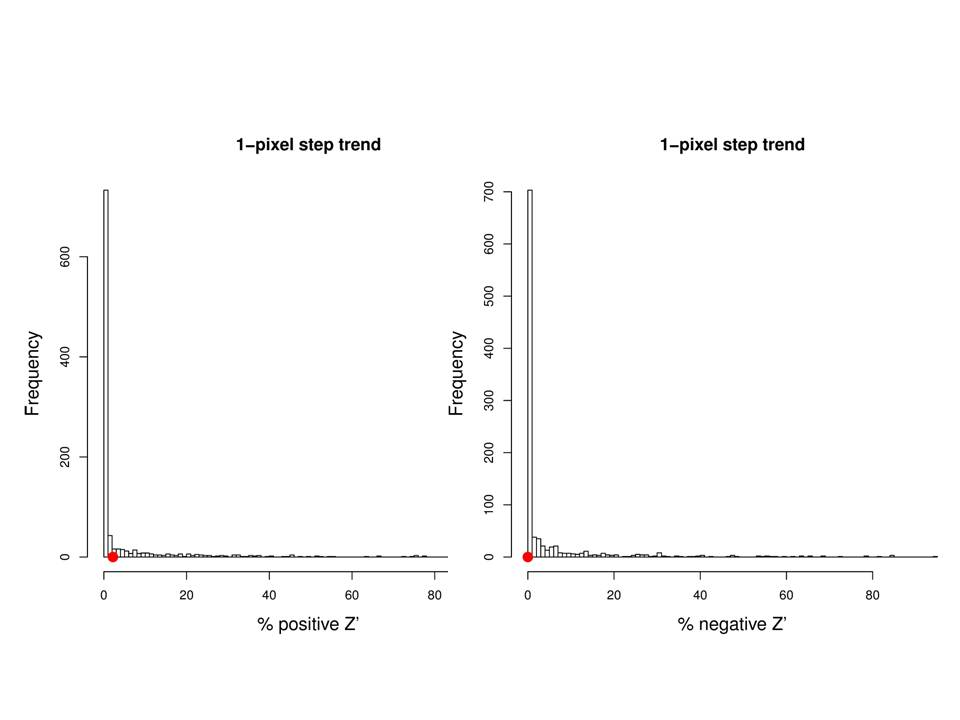
\includegraphics[width=6.5in]{bt1_nsw.jpg}
\caption{Percentage of pixels showing statistically significant positive Z' values (left) and negative Z' values (right) in NSW/VIC. The histogram shows the distribution of results from 1000 bootstrap resampling of the rainfall time series. The red dot represents the results from the observed data.}
\label{fig:boot_nsw}
\end{figure}


% chunk 8

\section{Summary and Discussion}

Generally, empirical studies on LCC-precipitation interaction are conducted within an area with known land surface intervention \citep[e.g.][]{Otterman1990,Durieux2003,Negri2004,Sato2007}. However, these locations are rare and difficult to isolate from real landscape change. In this study we therefore tested the effect of land cover change across a broad region, rather than only for locations where changes were known to occur or have occured. The advantage of this approach is that it does not require a long time series of land cover data which is usually unavailable. Furthermore, it does not assume a specific relationship between vegetation cover change and rainfall but allows the data to show this relationship, by applying the analysis to a broader area outside the boundary of the vegetation cover change. This approach is expected to provide a way to reduce the risk of a false positive paradox, by comparing results between areas with and without vegetation cover change. %On the other hand, this method is limited to step change analysis and cannot show a long term relationship. 

Parametric tests are generally more powerful than nonparametric test in detecting a trend, when the data is normally distributed \citep{Onoz2003,Kundzewicz2004}. As a non-parametric test, the step trend test has the advantages of distribution free and having no restriction on missing data \citep{Hirsch1985}. This is particularly useful in rainfall analysis since rainfall data is usually skewed. On the other hand, the disadvantages of non-parametric tests, such as being limited to hypothesis testing and weaker in power, also hold for the step trend test \citep{Whitley2002}. 

The regression model used here is a simple model. We only consider the important effects of historical trend, seasonality and climate drivers. Furthermore, no more than two large scale climatic indices were used in order to avoid over-parameterisation and multiple cross-correlations between climatic indices. A purpose of the regression model is to remove the variability in rainfall that is due to these known important factors. The model shows that seasonality, ENSO and IOD together explain no more than 20\% of the rainfall variability, and around 6 - 8\% on average is due to the climate drivers. This is consistent with the literature \citep[e.g.][]{Westra2010}. A large amount of variation is left in the model residuals, which is likely due to random factors. Rainfall is generally considered a stochastic process \citep[e.g.][]{Fowler2005,Cowpertwait2009,Burton2010}. The high variability increases the difficulty to detect a change in rainfall. 

There was some, but no strong evidence that a step change has occurred in the QLD region. The semi-parametric model could not identify any step change in the rainfall data. On the other hand, the step trend test suggested a couple of locations (300 - 500 km$^2$) might have experienced rainfall change ($\alpha = 0.05$). The results from the step trend test also indicated a possible widespread change, but the spatial pattern of change is not consistent with the tree cover change map. Although land clearings in QLD have occurred at a high rate and broad scale \citep{SLATS2005}, this study cannot confirm its impact on the local rainfall. At this location, land cover change was not found to change the mean rainfall significantly in some other studies \citep[e.g.][]{Narisma2003,McAlpine2007}. The characteristics of vegetation cover changes in QLD might increase the difficulty in detecting a step change. QLD has a long history of land clearing. According to the series of SLATS reports on land cover changes in QLD released by the Queensland government, land clearing continued in and around the study region between 1988 - 2008. Major broad scale and high rate clearings occurred in 1999 - 2000 and 2002 - 2004. It is therefore difficult to define a clear cut change in this region. The more continuous ongoing land clearing could have reduced the significance of a step change. %Furthermore, woodlands were mainly replaced by pasture after the clearing 
%% comment: Can we show that 2006 is an anomaly in the residuals?
The two methods indicate quite different results on the level of change in the NSW/VIC region. The semi-parametric model showed that a large area in the NSW/VIC region has experienced significant step change ($\alpha = 0.05$) in rainfall after 2003. But this result is likely to be affected by the low rainfall in 2006 as the area is larger than the bushfires region. The step trend test was able to detect significant changes ($\alpha = 0.05$) in about 400 km$^2$ areas in the Snowy Mt. and some possible changes along the bushfires region ($\alpha = 0.1$). This might be due to the possible small size of the step change and/or a short after-fire period \citep{Hirsch1985}. The vegetation cover change due to bushfires might have possibly changed the rainfall but the evidence was not strong either. 

%Both methods have highlighted the bushfires sites in the Snowy Mt. ranges. Especially in the step trend test results, a step change in rainfall in the bushfires locations is generally more significant than its surrounding regions. The step trend test results also suggested that the step change in rainfall, if any, had a  sign to the west of the bushfires area. This area corresponds to around 30\% of tree growth in the tree cover. This is evidence that the result of the step trend test is robust. 

The bushfires locations highlighted in the analysis results is an interesting outcome. The results might be due to a drought effect. The 2002 - 2003 drought has affected rainfall in a large part of Australia, particularly the MDB \citep{Nicholls2004}. The severe bushfires in 2003 were also triggered by the extreme drought conditions. Although the dry episode effect on rainfall has been accounted for in part by the SOI, further impact of drought could be passed through the local land-atmosphere interaction. However, this impact might not be statistically significant, even under an extreme event such as bushfires. Overall, the rainfall feedback to the vegetation cover change could be weak under the dry conditions. We found similar results in the later chapters.

The different causes of vegetation cover change in these two regions could lead to different post-change characteristics. The magnitude of EVI decreasing trends in the QLD region are less than in NSW region, as reported in the DLCD data. This is due to the lower tree density in the QLD region than in the NSW/VIC region before land surface interventions. Wild fires might have totally damaged the vegetation cover and recovery was very slow in some areas within the Snowy Mt. The persistent drought in the 2000s \citep{Howden2012} has delayed the regrowth of trees. On the other hand, replacing tree cover with pasture and crops might have a relatively subtle impact on the EVI. On the other hand, regrowth of trees can be expected after fires or as drought condition is relieved; but clearings for agricultural purpose impose permanent or semi-permanent changes to the land surface.

The rainfall data used in this study is a gridded data set. This data set is robust and consistent over a long time series (from 1900 to current) and has a broad national wide coverage which can provide more information spatially. However, high cross correlation between pixels due to the interpolation method generating this data set can also introduce spatial noise. Here the cross correlation has been account for in the step trend test. Some other methods are also available which can be used to perform a comparative trial. For example, \citet{Narisma2007} applied a spatial Gaussian filter on a similar data set and used wavelet analysis to detect step change in rainfall. High quality station data is another option to test whether the observed spatial pattern in the step trend test results was not due to the gridded data itself. Resampling methods, such as bootstrapping and permutation \citep{Wilks1997,Kundzewicz2004,Westra2013}, can also be used to further assess the strength of significance of results and incorporate spatial and temporal patterns in the analysis. We are also aware that the gridded data set is most useful in regions with sparse rain gauge networks but it actually reduces information where the rain gauge density is high \citep{Jones2009}. In the Snowy Mt. areas, the coverage of rainfall stations is intensive but they are mainly located in the valleys. The interpolated data might not best represent the local rainfall.

The current study cannot provide strong evidence to reject the null hypothesis (no step change in rainfall is due to the tree cover loss). Limiting by the available data, the time frame under study has been chosen within a long lasting drought period \citep{Holper2011}. The strong impact of this prolong drought might have suppressed the land-atmosphere interaction and confused the cause-effect relation between rainfall and vegetation cover change. This could be one of the reasons that the LCC effects found in other studies \citep[e.g.]{Gorgen2006,McAlpine2007} are not found to be significant here. So possible future work can be conducted for non-drought period, when longer series of land cover data is available. This approach should be further assessed in different scenarios of wet period and/or afforestation. Continuous monitoring of land surface conditions is important for future research. The power of the test can also be improved with the longer length of the after-intervention period \citep{Hirsch1985}. But then the question is what is an appropriate length for land cover change study, when ongoing change is possible, such as tree regrowth or cropping. This will require further research.

% \citet{Zhang2007} discover the relation in the way of map contras

% \citet{Webb2005} do not find a strong relationship between forest cover and total rainfall, which appears to be influenced primarily by factors such as distance to the coast; but significant positive relationships between tree cover and the number of rain days consistently emerge. 

%Both methods have identified some areas with rainfall change after the specified time of land cover change. This change in QLD appears to be less significant. Furthermore, the spatial distribution of significance of the changes do not well match with the tree cover change map. The results from the step trend test implied that a large scale change could have occurred, possibly due to the land clearing. The tree cover change map only shows a low level of changes (generally less than 20\%) spreading around the region between 2002 - 2005. The ongoing clearing activities in this region could be the reason that a step change cannot be detected. Both methods have better results in the NSW/VIC region, showing rainfall change in an area from the mountain range in the south to the west of ACT. The dummy variable is a significant predictor for rainfall in this area at the 0.05 level. In the step trend test the locations of bushfires is highlighted but the significance level is reduced. The two methods agree on the type of relationship. The regression analysis with dummy variable indicated that tree cover has a positive relationship with rainfall, while the step trend test showed that the tree cover loss might have decreased rainfall. However, the estimated relationship between land cover changes and the rainfall might not be highly significant. There is no strong evidence that the rainfall change is solely due to land cover change.

\section{Conclusion}

In this study, we found some evidence, although not strong, that vegetation cover change has changed local rainfall. The semi-parametric method and non-parametric method did not reach an agreement on detecting significant step change in rainfall in the hot dry QLD region where land clearing has occurred. On the other hand, the bushfires in the humid temperate mountain range in the NSW/VIC region could have reduced rainfall. But the dry spell also plays an important role in the results. 

Drought has had a pronounced impact on the land surface condition during the study period, leading to significant reduction in vegetation and extreme events such as bushfires. The lack of rainfall associated and high temperature may cause a step change in the vegetation. Hence, the signal of LCC feedback on rainfall is probably weaker under such regional dry condition, as the impact of LCC on rainfall is mainly through changes in moisture convergence \citep{Gorgen2006,Pitman2007}.


%Empirical evidence of correlations between rainfall and land cover change are scarce due to multiple environmental factors that cannot be controlled. In this study we investigated the relationship by applying statistical methods on data from best available sources. Gridded data of rainfall and tree cover were used as spatially corresponding local conditions. Large scale effects were represented by climatic indicators, such as SOI and IOD. Regression analysis and step trend tests were used to assess the effect of abrupt land surface intervention. 



%The step trend test is a better method than the regression method in this study. In order to obtain better results, the regression model requires fine details of the land covers. The defined land cover variable in the regression model does not significantly improve the model's reliability as the signal of change is smaller than the noise. Furthermore, the decrease of tree cover does not necessarily cause an immediate decrease in rainfall but it might alter the rainfall patterns or rainfall trend over the long term. While the regression analysis requires a long data record, the step trend test itself can work on a shorter data record. The step trend test can also achieve a better result than the regression analysis. Hence the step trend test is an easy and relatively reliable method to investigate the relationship between land cover changes and the rainfall when an abrupt change can be clearly identified. 

%The general information from the tree cover data can not support the assumption  In QLD, the continuous land clearing over more than a decade might provide some explanations to the results. The selected time window of land cover change could be unrealistic and the intensity of tree cover change in 2002 - 2005 is not climatically significant. On the other hand, results from step trend test on 1998 - 2008 rainfall data in NSW/VIC region has a better visual match with the tree cover change map, which indicates the method works better when a abrupt change can be clearly identified. The results from the step trend test on 11-year data implies a positive relationship between the tree covers and the rainfall at 0.1 significance level. This is a weak evidence that the loss of tree covers has led to rainfall decreasing.

%This study is a new attempt to use the step trend test in detecting rainfall change and attribute the result to specified land cover change. Comparing with the generalized additive regression method, this test does not require detailed information on land cover change but still achieves similar or even improved results. However, the relatively short length of rainfall data, especially there were only four to five years data after the specified intervention, has limited the performance of the test. Furthermore, equivalent long time series of good quality land cover data is also neccessary to investigate the history of vegetation cover change and identify the most significant events.

%----------------------------------------------------------------------------------------
%	APPENDICES (OPTIONAL)
%----------------------------------------------------------------------------------------

%%%%%%%%%%%%%%%%%%%%%%%%%%%%%%%%

\appendix

\section{Summary of Data}

 \begin{sidewaystable}
 \caption{Summary of data.}
  \label{tab:ch3Data}
 \begin{tabular}{lllll}
  \hline
  \textbf{Data} & \textbf{Source} & \multicolumn{2}{c}{\textbf{Resolution}} & \textbf{Analysis period} \\\cline{3-4}
  & & Temporal & Spatial & \\\hline
  Percent tree cover & MOD44B & Annual &	250m & 2000-2010\\
  Trend of vegetation cover change  &	DLCD (2009)	& Onetime & 250m	& Trend of Apr 2000 - Apr 2008\\
  Rainfall &	AWAP gridded rainfall data &	Monthly &	0.05\textdegree$\times$0.05\textdegree & Jan 1979- Dec 2008\\
  SOI	& BoM	& Monthly &	N/A &	Jan 1979- Dec 2008\\
  NINO 3, 3.4, 4 &	IRI/LDEO data library	& Monthly	& N/A	& Jan 1979- Dec 2008\\
  PDO	& NOAA & Monthly	& N/A	& Jan 1979- Dec 2008\\
  IOD	& POAMA-2 dataset	& Monthly	& N/A	& Jan 1979- Dec 2008\\
  \hline
  \end{tabular}
\end{sidewaystable}

%----------------------------------------------------------------------------------------
%	ACKNOWLEDGEMENTS
%----------------------------------------------------------------------------------------

\begin{acknowledgments}
CL was supported by an Australian Postgraduate Award for this work.
\end{acknowledgments}

%----------------------------------------------------------------------------------------
%	BIBLIOGRAPHY
%----------------------------------------------------------------------------------------

\bibliographystyle{agufull08}
\bibliography{reflist_chap3}

\end{article}

\end{document}











%% backup old code

% chunk 7

%The tree cover data is upscaled to match the resolution of the rainfall data. The upscaling process, taking the mean of pixel values, reduces the intensity of tree cover change, especially in the area where the change concentrates within small scale. Comparing the tree cover (as percentage of the ground area) in the QLD region between 2005 and 2002, light reduction of trees at the 5 km $\times$ 5 km resolution has been observed in the west and southwest of the region (Figure~\ref{fig:site1_tc}). In the NSW/VIC region, moderate to high tree cover change has shown along the MDB boundary (Figure~\ref{fig:site2_tc}). In the Snowy Mt. range, tree cover decreased between 2002 - 2003, while close to the southwest of ACT border there is increasing tree cover within the same period. 

%\begin{figure}[htp]
%  \centering
%  \mbox{\subfigure[site 1: tree cover change between 2002 & 2005]{\label{fig:site1_tc}\includegraphics[width=2.5in]{chap3/tc_qld.eps}}
%  \quad
%  \subfigure[site 2: tree cover change between 2002 & 2003 ]{\label{fig:site2_tc}\includegraphics[width=2.5in]{chap3/tc_nswvic.eps}}}
%  \caption{Tree cover change as percentage of ground area in the two study regions. Green colours indicate tree cover increase and pink colours indicate tree cover decrease.}
%  \label{fig:tc}
%\end{figure}

%The tree cover change map and the rainfall change map show some similarity in the NSW/VIC region. Positive values of Z' statistics (decreasing rainfall) in the Snowy Mountains correspond to tree cover reduction in 2002 - 2003. Around the higher Z' values (positive, significant at 10\%), the tree cover reduction is relatively more intense. However, where the increasing rainfall (significant at 10\%) is seen, the tree cover appears to be a mixture of small postive and negative changes which are less than 10\% of the ground area. 

% chunk 7

%Some of the land cover changes shown in Figure~\ref{fig:tc} are not significant, which means it might not be the largest land intervention or the change is not persistent. In Figure~\ref{fig:tc_z}, the relationship between the significant tree cover change and Z' value is shown. Here ''significant tree cover change" is defined as: difference of average tree cover between periods before and after intervention is over 5\% of ground area; and the variance in the after period is at most as much as the before period. A positive relationship refers to increasing (decreasing) rainfall (as represent by negative (positive) Z' value) associated with increasing (decreasing) land cover change. Otherwise it is negative relationship. There is limited number of pixels that have significant land cover changes in each region respectively. In the QLD region, these pixels all indicate tree cover reduction. there is about equal chance of positive relationship and negative relationship. In the NSW/VIC region, positive relationship is dominant. Around the Snowy Mt. range where tree cover was reduced, rainfall probably decrease too. On the other hand, in the middle of the region above Tumbarumba, tree cover increase is associated with possible increase trend in rainfall.

%\begin{figure}[htp]
%  \centering
%  \mbox{\subfigure[site 1: relationship between Z' value and sig. tree cover change]{\label{fig:site1_tcz}\includegraphics[width=2.5in]{tc_z_qld.eps}}
%  \quad
%  \subfigure[site 2: relationship between Z' value and sig. tree cover change ]{\label{fig:site2_tcz}\includegraphics[width=2.5in]{tc_z_nswvic.eps}}}
%  \caption{The maps show location where tree cover change is significant. Blue colour indicates the relationship between tree cover change and rainfall is positive (i.e. increasing tree cover and increasing rainfall or vice versa). Red colour indicates the relationship is negative.}
%  \label{fig:tc_z}
%\end{figure}


%\begin{figure}[htp]
%  \centering
%  \subfigure[QLD]{\label{fig:trend_qld}\includegraphics[height=2.5in]{"cv_trend1"}}
%  \subfigure[NSW/VIC]{\label{fig:trend_nsw}\includegraphics[height=1in,trim=0cm 5cm 0cm 5cm, clip=T]{"cv_trend2"}}
%  \subfigure[WA]{\label{fig:trend_wa}\includegraphics[height=1in,trim=0cm 11.5cm 0cm 1.5cm,clip=T]{"cv_trend3"}}  
%  \caption{Average annual rainfall (left), coefficient of variance (CV) of monthly rainfall (middle) and decadal rainfall change due to trend (right) for the three study regions. The area with significant trend (at $\alpha=0.05$ and $\alpha=0.1$) are also shown as an orange transparent patch on all the plots.}%
%  \label{fig:trend_rain}
%\end{figure}


%% supplement R code for other purpose

%% chunk 10
